\documentclass[../main.tex]{subfiles}
\begin{document}

\chapter{Boundary-Value Problems}

\begin{center}
    \Large{\textbf{CHAPTER OBJECTIVES}}
\end{center}
The primary objective of this chapter is to introduce you to solving boundary-value
problems for ODEs. Specific objectives and topics covered are
\begin{itemize}
    \item Understanding the difference between initial-value and boundary-value problems
    \item Knowing how to express an \textit{n}th-order ODE as a system of n first-order ODEs.
    \item Knowing how to implement the shooting method for linear ODEs by using linear
    interpolation to generate accurate ``shots.''
    \item Understanding how derivative boundary conditions are incorporated into the
    shooting method.
    \item Knowing how to solve nonlinear ODEs with the shooting method by using root
    location to generate accurate ``shots.''
    \item Knowing how to implement the finite-difference method.
    \item Understanding how derivative boundary conditions are incorporated into the
    finite-difference method.
    \item Knowing how to solve nonlinear ODEs with the finite-difference method by using
    root-location methods for systems of nonlinear algebraic equations.
\end{itemize}

\newpage

\noindent \large{\textbf{You've got a problem.}}

\noindent To this point, we have been computing the velocity of a free-falling bungee jumper by
integrating a single ODE:

\begin{equation}
    \tag{24.1}
    \frac{d v}{d t}=g-\frac{c_{d}}{m} v^{2}
\end{equation}

Suppose that rather than velocity, you are asked to determine the position of the jumper as
a function of time. One way to do this is to recognize that velocity is the first derivative of distance:

\begin{equation}
    \tag{24.2}
    \frac{dx}{dt} = v
\end{equation}

\noindent Thus, by solving the system of two ODEs represented by Eqs. (24.1) and (24.2), we can
simultaneously determine both the velocity and the position.

However, because we are now integrating two ODEs, we require two conditions to
obtain the solution. We are already familiar with one way to do this for the case where we
have values for both position and velocity at the initial time:

\begin{equation} \nonumber
    \begin{aligned}
    &x(t=0)=x_{i} \\
    &v(t=0)=v_{i}
    \end{aligned}
\end{equation}

\noindent Given such conditions, we can easily integrate the ODEs using the numerical techniques
described in Chaps. 22 and 23. This is referred to as an \textit{initial-value problem}.

But what if we do not know values for both position and velocity at $t = 0$? Let's say
that we know the initial position but rather than having the initial velocity, we want the
jumper to be at a specified position at a later time. In other words:
\begin{equation} \nonumber
    \begin{aligned}
        &x(t=0) = x_i \\
        &x(t=t_f) = x_f
    \end{aligned}
\end{equation}

\noindent Because the two conditions are given at different values of the independent variable, this is called a \textit{boundary-value problem}.
Such problems require special solution techniques. Some of these are related to the
methods for initial value problems that were described in the previous two chapters. However, others employ entirely different strategies to obtain solutions. This chapter is designed to introduce you to the more common of these methods.\vspace{2cm}

\section{Introduciton and background}

\subsection{What are Boundary-Value Problems?}

\noindent An ordinary differential equation is accompanied by auxiliary conditions, which are used
to evaluate the constants of integration that result during the solution of the equation. For
an \textit{n}th-order equation, \textit{n} conditions are required. If all the conditions are specified at the same value of the independent variable, then we are dealing with an \textit{initial-value problem} (Fig. 24.1\textit{a}). To this point, the material in Part Six (Chaps. 22 and 23) has been devoted to
this type of problem.

In contrast, there are often cases when the conditions are not known at a single point
but rather are given at different values of the independent variable. Because these values
are often specified at the extreme points or boundaries of a system, they are customarily
referred to as \textit{boundary-value problems} (Fig. 24.1\textit{b}). A variety of significant engineering applications fall within this class. In this chapter, we discuss some of the basic approaches for solving such problems.

\begin{figure}[H]
    \centering
    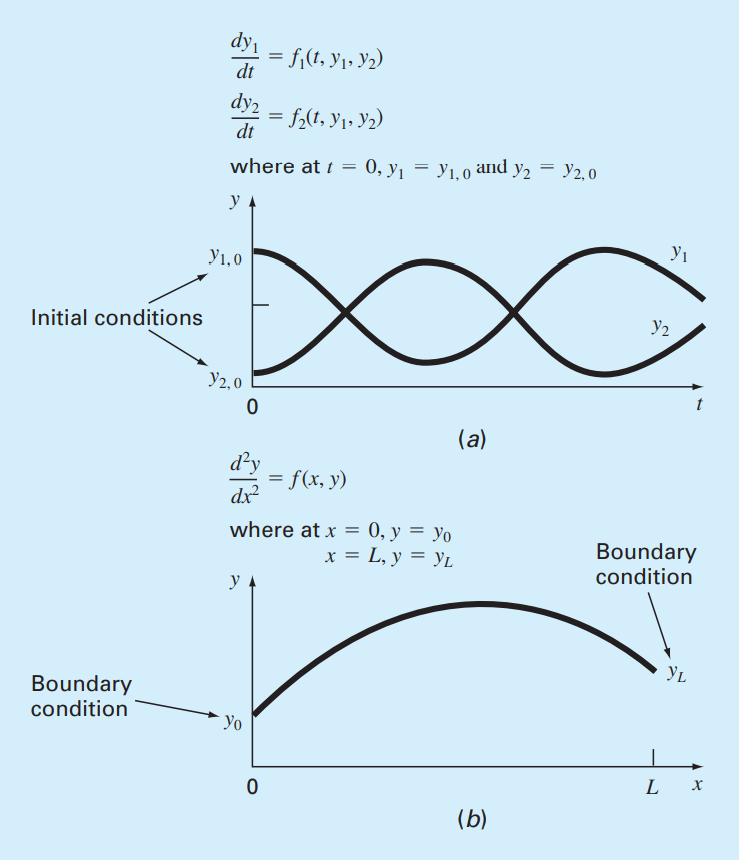
\includegraphics[scale=0.4]{fig_24_1}
   \caption{\textsf{Initial-value versus boundary-value problems. (a) An initial-value problem where all the conditions
   are specified at the same value of the independent variable. (b) A boundary-value problem
   where the conditions are specified at different values of the independent variable.}}\label{fig:fig_24_1}
\end{figure}

\subsection{Boundary-Value Problems in Engineering and Science}

\noindent At the beginning of this chapter, we showed how the determination of the position and velocity of a falling object could be formulated as a boundary-value problem. For that example, a pair of ODEs was integrated in time. Although other time-variable examples can be
developed, boundary-value problems arise more naturally when integrating in space. This
occurs because auxiliary conditions are often specified at different positions in space.

A case in point is the simulation of the steady-state temperature distribution for a long,
thin rod positioned between two constant-temperature walls (Fig. 24.2). The rod's crosssectional dimensions are small enough so that radial temperature gradients are minimal
and, consequently, temperature is a function exclusively of the axial coordinate x. Heat is
transferred along the rod's longitudinal axis by conduction and between the rod and the
surrounding gas by convection. For this example, radiation is assumed to be negligible.
\footnote[1]{We incorporate radiation into this problem later in this chapter in Example 24.4.}

\begin{figure}[H]
    \centering
    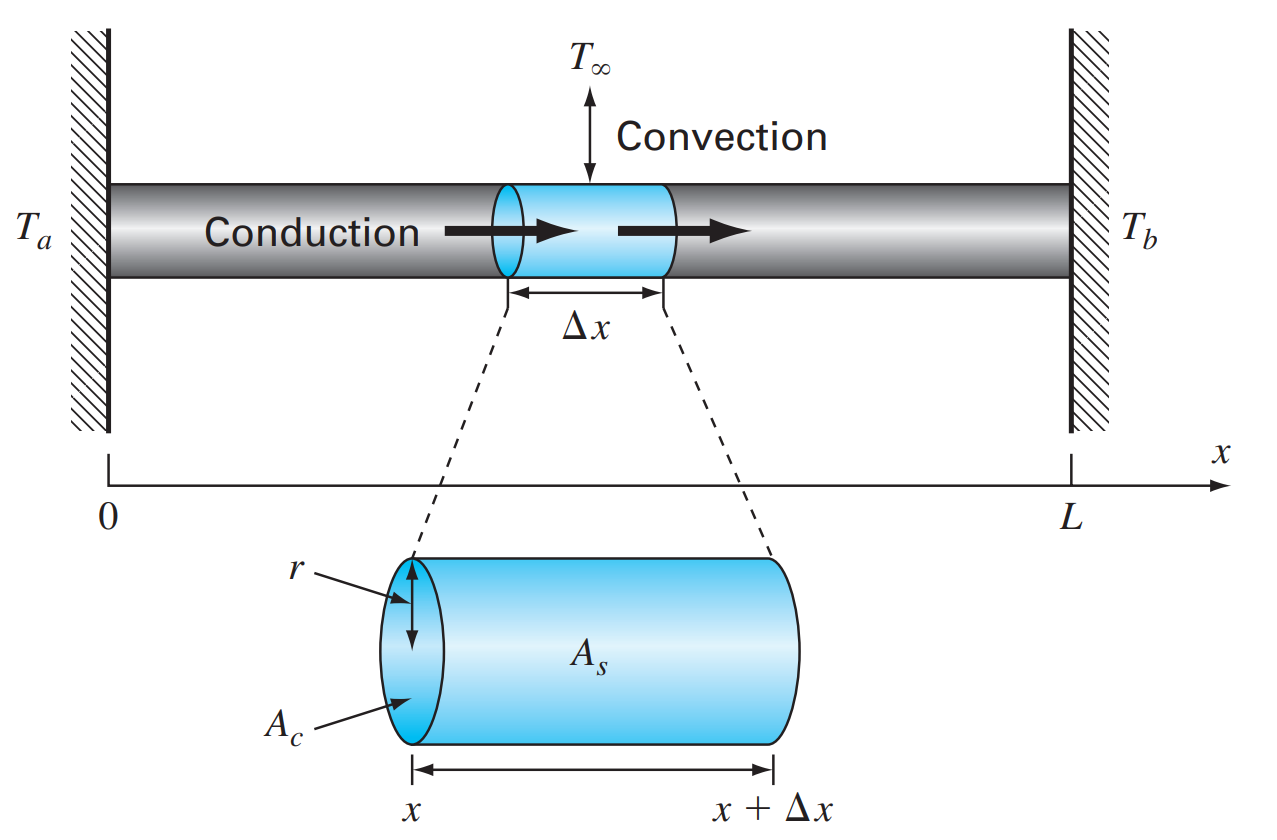
\includegraphics[scale=0.3]{fig_24_2}
   \caption{\textsf{A heat balance for a differential element of a heated rod subject to conduction and convection.}}\label{fig:fig_24_2}
\end{figure}

As depicted in Fig. 24.2, a heat balance can be taken around a differential element of thickness $\Delta x$ as
\begin{equation}
    \tag{24.3}
    0=q(x) A_{c}-q(x+\Delta x) A_{c}+h A_{s}\left(T_{\infty}-T\right)
\end{equation}

\noindent where $q(x)=$ flux into the element due to conduction $\left[\mathrm{J} /\left(\mathrm{m}^{2} \cdot \mathrm{s}\right)\right] ; q(x+\Delta x)=$ flux out of the element due to conduction $\left[\mathrm{J} /\left(\mathrm{m}^{2} \cdot \mathrm{s}\right)\right] ; A_{c}=$ cross-sectional area
$\left[\mathrm{m}^{2}\right]=\pi r^{2}, r=$ the radius $[\mathrm{m}] ; h=$ the convection heat transfer coefficient $\left[\mathrm{J} /\left(\mathrm{m}^{2} \cdot \mathrm{K} \cdot \mathrm{s}\right)\right] ; A_{s}=$ the element's surface area $\left[\mathrm{m}^{2}\right]=2 \pi r \Delta x ; T_{\infty}=$ the temperature of the surrounding gas $[\mathrm{K}]$; and $T=$ the rod's temperature $[\mathrm{K}]$.

Equation (24.3) can be divided by the element's volume $\left(\pi r^{2} \Delta x\right)$ to yield
$$
0=\frac{q(x)-q(x+\Delta x)}{\Delta x}+\frac{2 h}{r}\left(T_{\infty}-T\right)
$$
Taking the limit $\Delta x \rightarrow 0$ gives
\begin{equation}
    \tag{24.4}
    0=-\frac{d q}{d x}+\frac{2 h}{r}\left(T_{\infty}-T\right)
\end{equation}

\noindent The flux can be related to the temperature gradient by Fourier's law:
\begin{equation}
    \tag{24.5}
    q=-k \frac{d T}{d x}
\end{equation}

\noindent where $k=$ the coefficient of thermal conductivity $[\mathrm{J} /(\mathrm{s} \cdot \mathrm{m} \cdot \mathrm{K})]$. Equation $(24.5)$ can be differentiated with respect to $x$, substituted into Eq. (24.4), and the result divided by $k$ to yield,
\begin{equation}
    \tag{24.6}
    0=\frac{d^{2} T}{d x^{2}}+h^{\prime}\left(T_{\infty}-T\right)
\end{equation}

\noindent where $h^{\prime}=$ a bulk heat-transfer parameter reflecting the relative impacts of convection and conduction $\left[\mathrm{m}^{-2}\right]=2 h /(r k)$.

Equation (24.6) represents a mathematical model that can be used to compute the temperature along the rod's axial dimension. Because it is a second-order ODE, two conditions are required to obtain a solution. As depicted in Fig. 24.2, a common case is where the temperatures at the ends of the rod are held at fixed values. These can be expressed mathematically as

\begin{equation} \nonumber
    \begin{aligned}
        &T(0)=T_a\\
        &T(L)=T_b
    \end{aligned}
\end{equation}

\noindent The fact that they physically represent the conditions at the rod's ``boundaries'' is the origin of the terminology: boundary conditions.

Given these conditions, the model represented by Eq. (24.6) can be solved. Because
this particular ODE is linear, an analytical solution is possible as illustrated in the following example.

\begin{exmp}
    \textbf{Analytical Solution for a Heated Rod}

    \noindent \textit{Problem statement} Use calculus to solve Eq. (24.6) for a $10-\mathrm{m}$ rod with $h'= 0.005m^{-2}[h=1 J/(m^2\cdot K\cdot s)]$, $r=0.2\ m$, $k=200J/(s\cdot m\cdot K)]$, $T_\infty=200K$ and the boundary conditions:
    $$
    T(0)=300 \mathrm{~K} \quad T(10)=400 \mathrm{~K}
    $$
    \textbf{Solution.} This ODE can be solved in a number of ways. A straightforward approach is to first express the equation as
    $$
    \frac{d^{2} T}{d x^{2}}-h^{\prime} T=-h^{\prime} T_{\infty}
    $$
    Because this is a linear ODE with constant coefficients, the general solution can be readily obtained by setting the right-hand side to zero and assuming a solution of the form $T=e^{\lambda x}$. Substituting this solution along with its second derivative into the homogeneous form of the ODE yields
    $$
    \lambda^{2} e^{\lambda x}-h^{\prime} e^{\lambda x}=0
    $$
    which can be solved for $\lambda=\pm \sqrt{h^{\prime}}$. Thus, the general solution is
    $$
    T=A e^{\lambda x}+B e^{-\lambda x}
    $$
    where $A$ and $B$ are constants of integration. Using the method of undetermined coefficients we can derive the particular solution $T=T_{\infty}$. Therefore, the total solution is
    $$
    T=T_{\infty}+A e^{\lambda x}+B e^{-\lambda x}
    $$
    The constants can be evaluated by applying the boundary conditions
    $$
    \begin{aligned}
    &T_{a}=T_{\infty}+A+B \\
    &T_{b}=T_{\infty}+A e^{\lambda L}+B e^{-\lambda L}
    \end{aligned}
    $$
    These two equations can be solved simultaneously for
    $$
    \begin{aligned}
    &A=\frac{\left(T_{a}-T_{\infty}\right) e^{-\lambda L}-\left(T_{b}-T_{\infty}\right)}{e^{-\lambda L}-e^{\lambda L}} \\
    &B=\frac{\left(T_{b}-T_{\infty}\right)-\left(T_{a}-T_{\infty}\right) e^{\lambda L}}{e^{-\lambda L}-e^{\lambda L}}
    \end{aligned}
    $$

    \begin{figure}[H]
        \centering
        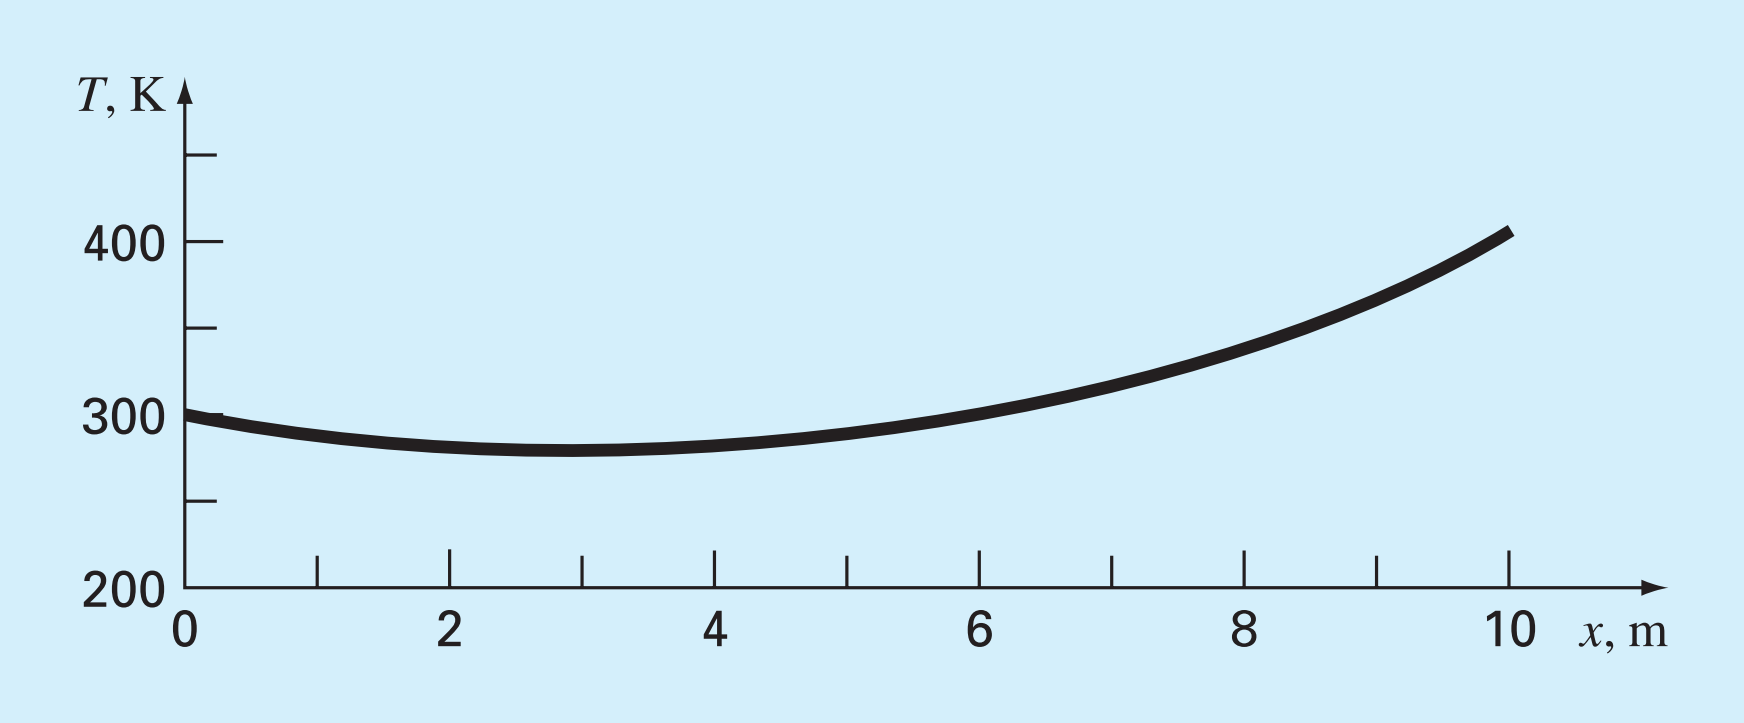
\includegraphics[scale=0.3]{fig_24_3}
       \caption{\textsf{Analytical solution for the heated rod.}}\label{fig:fig_24_3}
    \end{figure}

    \noindent Substituting the parameter values from this problem gives $A=20.4671$ and $B=$ 79.5329. Therefore, the final solution is
    \begin{equation}
        \tag{24.7}
        T=200+20.4671 e^{\sqrt{0.05} x}+79.5329 e^{-\sqrt{0.05} x}
    \end{equation}
    
    As can be seen in Fig. 24.3, the solution is a smooth curve connecting the two boundary temperatures. The temperature in the middle is depressed due to the convective heat loss to the cooler surrounding gas.
\end{exmp}\vspace{5mm}

In the following sections, we will illustrate numerical approaches for solving the same
problem we just solved analytically in Example 24.1. The exact analytical solution will be
useful in assessing the accuracy of the solutions obtained with the approximate, numerical
methods. \vspace{2cm}


\section{The Shooting Method}

\noindent The shooting method is based on converting the boundary-value problem into an equivalent initial-value problem. A trial-and-error approach is then implemented to develop a solution for the initial-value version that satisfies the given boundary conditions.

Although the method can be employed for higher-order and nonlinear equations, it is
nicely illustrated for a second-order, linear ODE such as the heated rod described in the
previous section:

\begin{equation}
    \tag{24.8}
    0=\frac{d^2T}{dx^2}+h'(T_\infty-T)
\end{equation}

\noindent subject to boundary conditions:

\begin{equation} \nonumber
    \begin{aligned}
        &T(0)=T_a\\
        &T(L)=T_b
    \end{aligned}
\end{equation}

We convert this boundary-value problem into an initial-value problem by defining the
rate of change of temperature, or \textit{gradient}, as

\begin{equation}
    \tag{24.9}
    \frac{d T}{d x}=z
\end{equation}

and reexpressing Eq. (24.8) as
\begin{equation}
    \tag{24.10}
    \frac{d z}{d x}=-h^{\prime}\left(T_{\infty}-T\right)
\end{equation}

\noindent Thus, we have converted the single second-order equation (Eq. 24.8) into a pair of firstorder ODEs (Eqs. $24.9$ and 24.10).

If we had initial conditions for both $T$ and $z$, we could solve these equations as an initialvalue problem with the methods described in Chaps. 22 and 23 . However, because we only have an initial value for one of the variables $T(0)=T_{a}$ we simply make a guess for the other $z(0)=z_{a 1}$ and then perform the integration.

After performing the integration, we will have generated a value of $T$ at the end of the interval, which we will call $T_{b 1}$. Unless we are incredibly lucky, this result will differ from the desired result $T_{b}$.

Now, let's say that the value of $T_{b 1}$ is too high $\left(T_{b 1}>T_{b}\right)$, it would make sense that a lower value of the initial slope $z(0)=z_{a 2}$ might result in a better prediction. Using this new guess, we can integrate again to generate a second result at the end of the interval $T_{b 2}$. We could then continue guessing in a trial-and-error fashion until we arrived at a guess for $z(0)$ that resulted in the correct value of $T(L)=T_{b}$.

At this point, the origin of the name shooting method should be pretty clear. Just as you would adjust the angle of a cannon in order to hit a target, we are adjusting the trajectory of our solution by guessing values of $z(0)$ until we hit our target $T(L)=T_{b}$.

Although we could certainly keep guessing, a more efficient strategy is possible for linear ODEs. In such cases, the trajectory of the perfect shot $z_{a}$ is linearly related to the results of our two erroneous shots $\left(z_{a 1}, T_{b 1}\right)$ and $\left(z_{a 2}, T_{b 2}\right)$. Consequently, linear interpolation can be employed to arrive at the required trajectory:
\begin{equation}
    \tag{24.11}
    z_{a}=z_{a 1}+\frac{z_{a 2}-z_{a 1}}{T_{b 2}-T_{b 1}}\left(T_{b}-T_{b 1}\right)
\end{equation}

The approach can be illustrated by an example.

\begin{exmp}
    \textbf{The Shooting Mehtod for a Linear ODE}

    \noindent \textit{Problem Statement.} Use the shooting method to solve Eq. (24.6) for the same coditions as Example 24.1: $L=10m$, $h'=0.005m^{-2}$, $T_\infty=200K$, $T(0)=300K$, and $T(10)=400K.$

    \noindent \textbf{Solution.} Equation (24.6) is first expressed as a pair of first-order ODEs:

    $$
    \begin{aligned}
    &\frac{d T}{d x}=z \\
    &\frac{d z}{d x}=-0.05(200-T)
    \end{aligned}
    $$
    Along with the initial value for temperature $T(0)=300 \mathrm{~K}$, we arbitrarily guess a value   of $z_{a 1}=-5 \mathrm{~K} / \mathrm{m}$ for the initial value for $z(0)$. The solution is then   obtained by integrating the pair of ODEs from $x=0$ to 10. We can do this with MATLAB's \texttt{ode45} function by first setting up an M-file to hold the differential equations:

    \noindent\texttt{function dy=Ex2402(x,y)\\
    dy=[y(2);-0.05*(200-y(l))];}

    \noindent We can then generate the solution as:

    \noindent\texttt{>> [t,y]=ode45(@Ex2402,[0 10],[300,-5]);\\
    >> Tb1=y(length(y))}

    \noindent\texttt{Tb1 =\\
    \vspace{\smallskipamount} 569.7539}

    \noindent Thus, we obtain a value at the end of the interval of $T_{b 1}=569.7539$ (Fig. $24.4 a$ ), which differs from the desired boundary condition of $T_{b}=400$. Therefore, we make another guess $z_{a 2}=-20$ and perform the computation again. This time, the result of $T_{b 2}=259.5131$ is obtained (Fig. 24.4b).

    \begin{figure}[H]
        \centering
        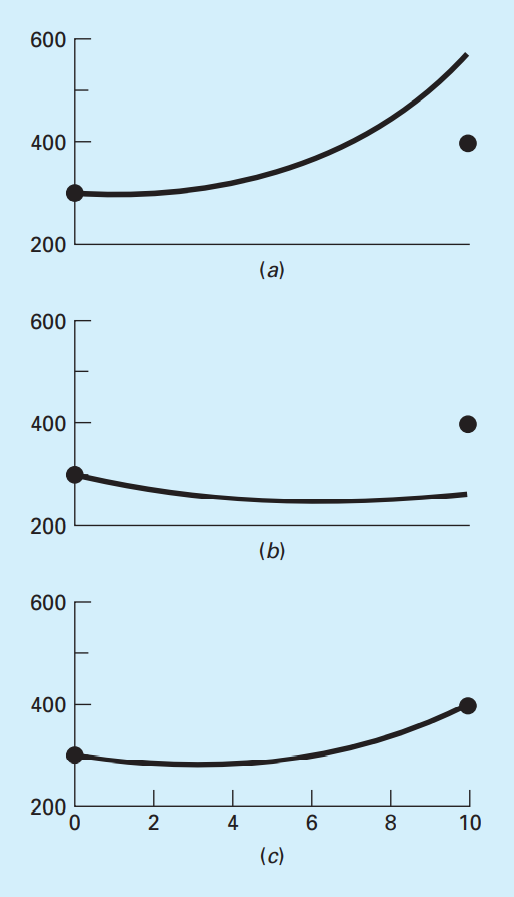
\includegraphics[scale=0.45]{fig_24_4}
       \caption{\textsf{Temperature (K) versus distance (m) computed with the shooting method: (a) the first ``shot,`` 
       (b) the second ``shot,`` and (c) the final exact ``hit.``}}\label{fig:fig_24_4}
    \end{figure}

    Now, because the original ODE is linear, we can use Eq. (24.11) to determine the correct trajectory to yield the perfect shot:
    $$
    z_{a}=-5+\frac{-20-(-5)}{259.5131-569.7539}(400-569.7539)=-13.2075
    $$
    \noindent This value can then be used in conjunction with \texttt{ode45} to generate the correct solution, asdepicted in Fig. 24.4c.

    Although it is not obvious from the graph, the analytical solution is also plotted on Fig. 24.4c. Thus, the shooting method yields a solution that is virtually indistinguishable from the exact result.
\end{exmp}

\subsection{Deriative Boundry Conditions}

The fixed or Dirichlet boundary condition discussed to this point is but one of several types
that are used in engineering and science. A common alternative is the case where the derivative is  given. This is commonly referred to as a Neumann boundary condition.
Because it is already set up to compute both the dependent variable and its derivative,
incorporating derivative boundary conditions into the shooting method is relatively
straightforward.
Just as with the fixed-boundary condition case, we first express the second-order ODE
as a pair of first-order ODEs. At this point, one of the required initial conditions, whether
the dependent variable or its derivative, will be unknown. Based on guesses for the missing initial condition, we generate solutions to compute the given end condition. As with the
initial condition, this end condition can either be for the dependent variable or its derivative. For linear ODEs, interpolation can then be used to determine the value of the missing
initial condition required to generate the final, perfect "shot" that hits the end condition.

\begin{exmp}
    \textbf{The Shooting Method with Derivative Boundary Conditions}

    \noindent\textit{Problem statement.} Use the shooting method to solve Eq. (24.6) for the rod in Example 24.1: $L=10 \mathrm{~m},\ h^{\prime}=0.05 \mathrm{~m}^{-2}\left[h=1 \mathrm{~J} /\left(\mathrm{m}^{2} \cdot \mathrm{K} \cdot \mathrm{s}\right),\ r=0.2 \mathrm{~m},\ k=200 \mathrm{~J} /\right.$ $(\mathrm{s} \cdot \mathrm{m} \cdot \mathrm{K})],\ T_{\infty}=200 \mathrm{~K}$, and $T(10)=400 \mathrm{~K}$.
    However, for this case, rather than having a fixed temperature of $300 \mathrm{~K}$, the left end is subject to convection as in Fig. 24.5. For simplicity, we will assume that the convection heat transfer coefficient for the end area is the same as for the rod's surface.

    \begin{figure}[H]
        \centering
        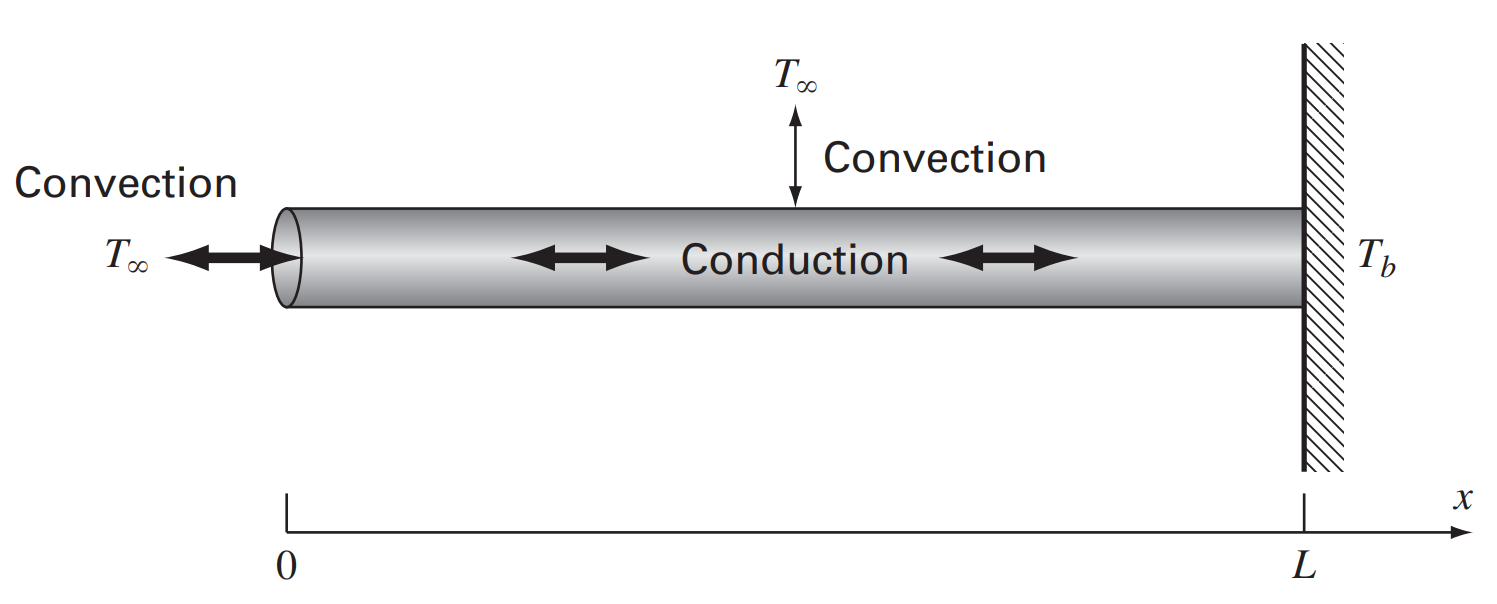
\includegraphics[scale=0.3]{fig_24_5}
       \caption{\textsf{A rod with a convective boundary condition at one end and a fixed temperature at the other.}}\label{fig:fig_24_5}
    \end{figure}
    \noindent\textbf{Solution.} As in Example 24.2, Eq. (24.6) is first expressed as

    $$
    \begin{aligned}
    &\frac{d T}{d x}=z \\
    &\frac{d z}{d x}=-0.05(200-T)
    \end{aligned}
    $$

    Although it might not be obvious, convection through the end is equivalent to specifying a gradient boundary    condition. In order to see this, we must recognize that because the system is at steady state, convection must equal conduction at the rod's left boundary $(x=0)$. Using Fourier's law (Eq. 24.5) to represent conduction, the heat balance at the end can be formulated as
    \begin{equation}
        \tag{24.12}
        h A_{c}\left(T_{\infty}-T(0)\right)=-k A_{c} \frac{d T}{d x}(0)
    \end{equation}
    
    This equation can be solved for the gradient
    \begin{equation}
        \tag{24.13}
        \frac{d T}{d x}(0)=\frac{h}{k}\left(T(0)-T_{\infty}\right)
    \end{equation}
    
    \noindent If we guess a value for temperature, we can see that this equation specifies the gradient.

    Theshooting method is implemented by arbitrarily guessing a value for $T(0)$. If we choose a value of $T(0)=T_{a 1}=300 \mathrm{~K}$, Eq. (24.13) then yields the initial value for the gradient
    $$
    z_{a 1}=\frac{d T}{d x}(0)=\frac{1}{200}(300-200)=0.5
    $$
    The solution is obtained by integrating the pair of ODEs from $x=0$ to 10 . We can do this with MATLAB's \texttt{ode45} function by first setting up an M-file to hold the differential equations in the same fashion as in Example 24.2. We can then generate the solution as

    \noindent\texttt{>> [t,y]=ode45(@Ex2402,[0 10],[300,0.5]);\\
    >> Tb1=y(length(y))}

    \noindent\texttt{Tb1 =\\
    \vspace{\smallskipamount} 683.5088}

    As expected, the value at the end of the interval of $T_{b1} = 683.5088 K$ differs from the
    desired boundary condition of $T_b = 400$. Therefore, we make another guess $T_{a2} = 150 K$,
    which corresponds to $z_{a2} = -0.25$, and perform the computation again.

    \noindent\texttt{>> [t,y]=ode45(@Ex2402,[0 10],[150,-0.25]);\\
    >> Tb2=y(length(y))}

    \noindent\texttt{Tb2 =\\
    \vspace{\smallskipamount} -41.7544}

    \begin{figure}[H]
        \centering
        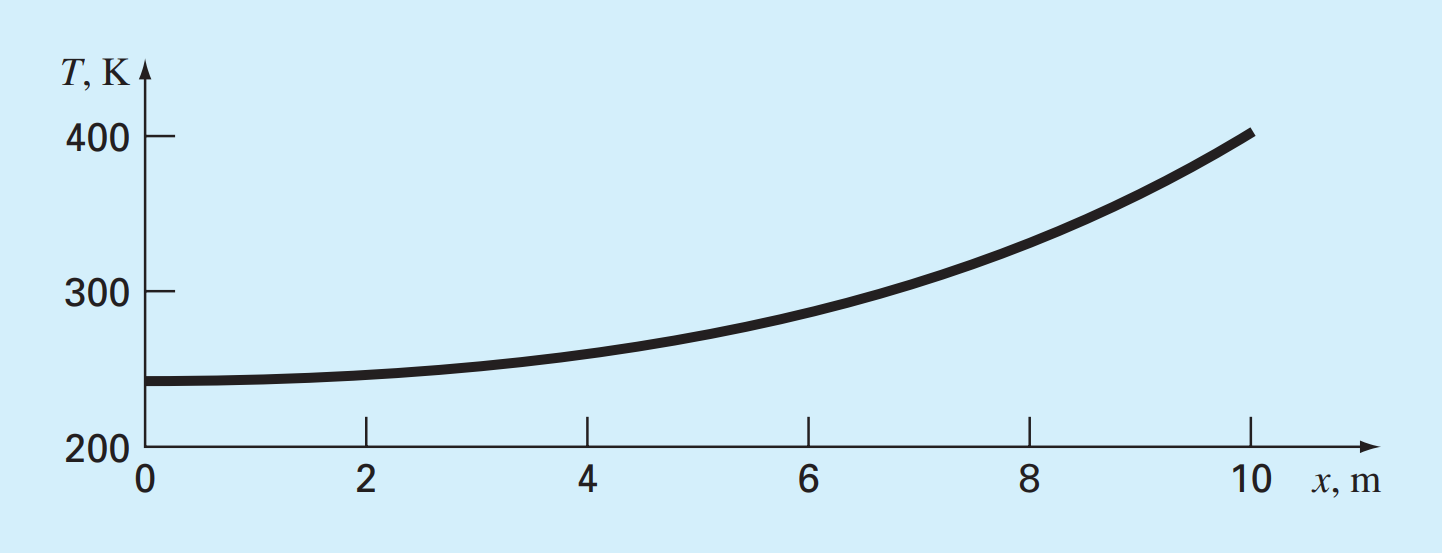
\includegraphics[scale=0.3]{fig_24_6}
       \caption{\textsf{The solution of a second-order ODE with a convective boundary condition at one end and a
       fixed temperature at the other.}}\label{fig:fig_24_6}
    \end{figure}

    \noindent Linear interpolation can then be employed to compute the correct initial temperature:
    $$
    T_{a}=300+\frac{150-300}{-41.7544-683.5088}(400-683.5088)=241.3643 \mathrm{~K}
    $$
    which corresponds to a gradient of $z_{a}=0.2068$. Using these initial conditions, \texttt{ode45} can be employed to generate the correct solution, as depicted in Fig. 24.6.

    Note that we can verify that our boundary condition has been satisfied by substituting the initial conditions into Eq. (24.12) to give
    $$
    1 \frac{\mathrm{J}}{\mathrm{m}^{2} \mathrm{~K} \mathrm{~s}} \pi \times(0.2 \mathrm{~m})^{2} \times(200 \mathrm{~K}-241.3643 \mathrm{~K})=-200 \frac{\mathrm{J}}{\mathrm{m} \mathrm{K} \mathrm{s}} \pi \times(0.2 \mathrm{~m})^{2} \times 0.2068 \frac{\mathrm{K}}{\mathrm{m}}
    $$
    which can be evaluated to yield $-5.1980 \mathrm{~J} / \mathrm{s}=-5.1980 \mathrm{~J} / \mathrm{s}$. Thus, conduction and convection are equal and transfer heat out of the left end of the rod at a rate of $5.1980 \mathrm{~W}$.
\end{exmp}

\subsection{The Shooting Method for Nonlinear ODEs}

\noindent For nonlinear boundary-value problems, linear interpolation or extrapolation through two solution points will not necessarily result in an accurate estimate of the required boundary condition to attain an exact solution. An alternative is to perform three applications of the shooting method and use a quadratic interpolating polynomial to estimate the proper boundary condition.
However, it is unlikely that such an approach would yield the exact answer, and additional iterations would be necessary to home in on the solution.

Another approach for a nonlinear problem involves recasting it as a roots problem. Recall that the general goal of a roots problem is to find the value of $x$ that makes the function $f(x)=0$. Now, let us use the heated rod problem to understand how the shooting method can be recast in this form.

First, recognize that the solution of the pair of differential equations is also a "function" in the sense that we guess a condition at the left-hand end of the rod $z_{a}$, and the integration yields a prediction of the temperature at the right-hand end $T_{b}$. Thus, we can think of the integration as
$$
T_{b}=f\left(z_{a}\right)
$$

\noindent That is, it represents a process whereby a guess of $z_{a}$ yields a prediction of $T_{b}$. Viewed in this way, we can see that what we desire is the value of $z_{a}$ that yields a specific value of $T_{b}$. If, as in the example, we desire $T_{b}=400$, the problem can be posed as
$$
400=f\left(z_{a}\right)
$$
By bringing the goal of 400 over to the right-hand side of the equation, we generate a new function res $\left(z_{a}\right)$ that represents the difference, or \textit{residual}, between what we have, $f\left(z_{a}\right)$, and what we want, 400.
$$
\operatorname{res}\left(z_{a}\right)=f\left(z_{a}\right)-400
$$
If we drive this new function to zero, we will obtain the solution. The next example illustrates the approach.

\begin{exmp}
    \textbf{The Shooting Method for Nonlinear ODEs}

    \noindent\textit{Problem statement.} Although it served our purposes for illustrating the shooting method, Eq. (24.6) was not a completely realistic model for a heated rod. For one thing, such a rod would lose heat by mechanisms such as radiation that are nonlinear.

    Suppose that the following nonlinear ODE is used to simulate the temperature of the heated rod:
    $$
    0=\frac{d^{2} T}{d x^{2}}+h^{\prime}\left(T_{\infty}-T\right)+\sigma^{\prime^{\prime}}\left(T_{\infty}^{4}-T^{4}\right)
    $$
    where $\sigma^{\prime}=$ a bulk heat-transfer parameter reflecting the relative impacts of radiation and conduction $=2.7 \times 10^{-9} \mathrm{~K}^{-3} \mathrm{~m}^{-2}$. This equation can serve to illustrate how the shooting method is used to solve a two-point nonlinear boundary-value problem. The remaining problem conditions are as specified in Example 24.2: $L=10 \mathrm{~m},\ h^{\prime}=0.05 \mathrm{~m}^{-2}$,\ $T_{\infty}=200 \mathrm{~K},\ T(0)=300 \mathrm{~K}$, and $T(10)=400 \mathrm{~K}$.
    
    \noindent\textbf{Solution.} Just as with the linear ODE, the nonlinear second-order equation is first expressed as two first-order ODEs:
    $$
    \begin{aligned}
    &\frac{d T}{d x}=z \\
    &\frac{d z}{d x}=-0.05(200-T)-2.7 \times 10^{-9}\left(1.6 \times 10^{9}-T^{4}\right)
    \end{aligned}
    $$
    An M-file can be developed to compute the right-hand sides of these equations:\vspace*{\smallskipamount}

    \noindent\texttt{function dy=dydxn(x,y)\\
    dy=[y(2);-0.05*(200-y(1))-2.7e-9*(1.6e9-y(1)\^{}4)];}\vspace*{\smallskipamount}

    \noindent Next, we can build a function to hold the residual that we will try to drive to zero as\vspace*{\smallskipamount}

    \noindent\texttt{function r=res(za)}\\
    \texttt{[x,y]=ode45(@dydxn,[0 10],[300 za]);\\
    r=y(length(x),1)-400;}

    \begin{figure}[H]
        \centering
        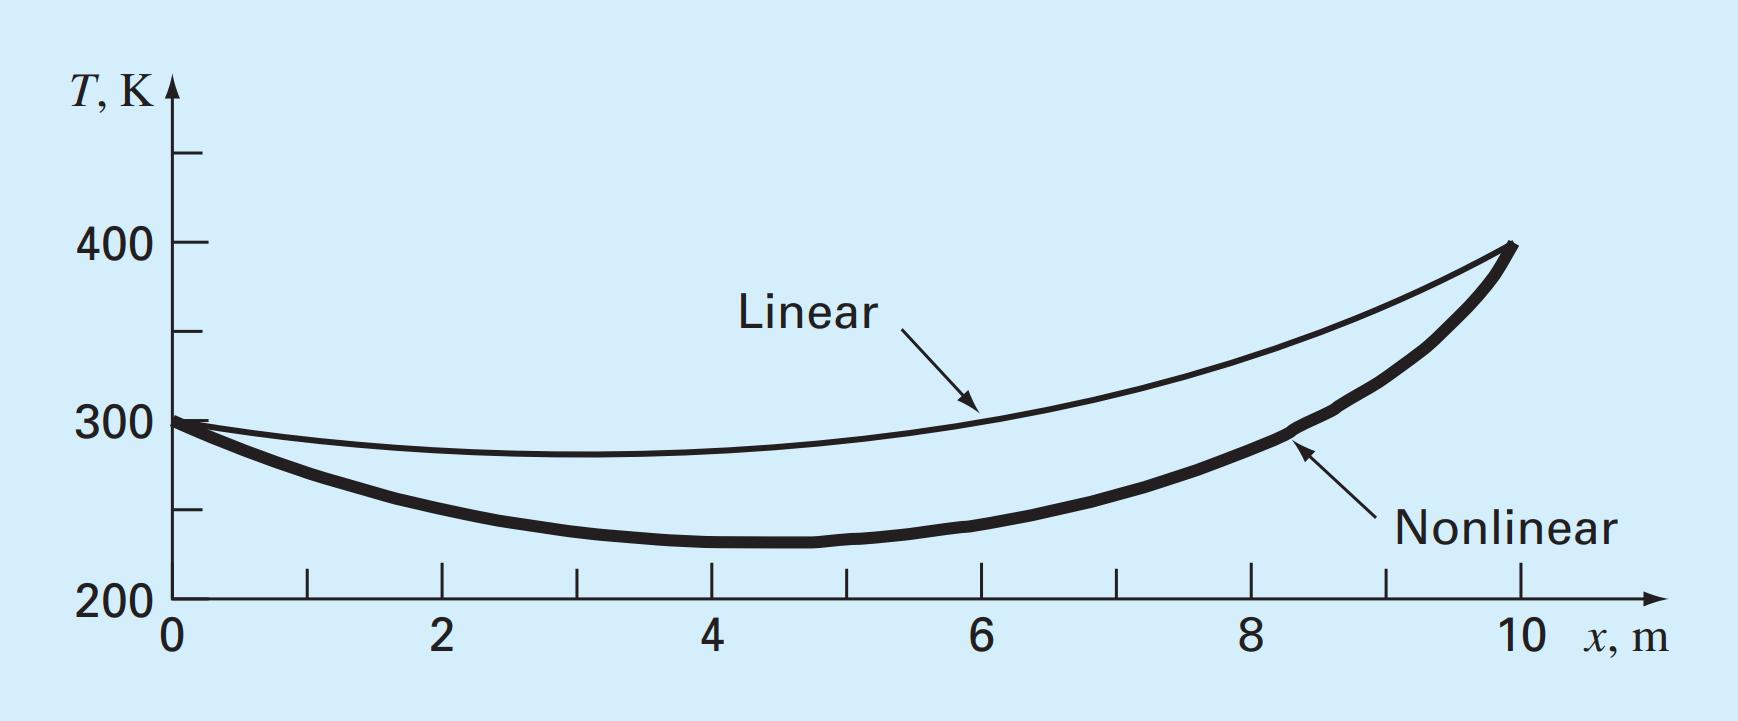
\includegraphics[scale=0.3]{fig_24_7}
       \caption{\textsf{The result of using the shooting method to solve a nonlinear problem.}}\label{fig:fig_24_7}
    \end{figure}
    \noindent Notice how we use the \texttt{ode45} function to solve the two ODEs to generate the temperature
    at the rod;s end: \texttt{y(length(x),1)}. We can then find the root with the \texttt{fzero} function:

    \noindent\texttt{>> fzero(@res,-50)}\vspace{\medskipamount}\\
    \texttt{ans =\\
    \hspace*{\smallskipamount} -41.7434}

    \noindent Thus, we see that if we set the initial trajectory $z(0)$ = -41.7434, the residual function will
    be driven to zero and the temperature boundary condition $T(10)$ = 400 at the end of the
    rod should be satisfied. This can be verified by generating the entire solution and plotting
    the temperatures versus x:\vspace*{\smallskipamount}

    \noindent\texttt{>> [x,y]=ode45(@dydxn,[0 10],[300 fzero(@res,-50)]);\\
    >> plot(x,y(:,1))}\vspace*{\smallskipamount}

    The result is shown in Fig. 24.7 along with the original linear case from Example 24.2.
    As expected, the nonlinear case is depressed lower than the linear model due to the additional heat lost to the surrounding gas by radiation.
\end{exmp}\vspace{2cm}

\section{Finite-Difference Methods}
\noindent The most common alternatives to the shooting method are finite-difference approaches. In
these techniques, finite differences (Chap. 21) are substituted for the derivatives in the
original equation. Thus, a linear differential equation is transformed into a set of simultaneous algebraic equations that can be solved using the methods from Part Three.

We can illustrate the approach for the heated rod model (Eq. 24.6):

\begin{equation}
    \tag{24.14}
    0=\frac{d^2T}{dx^2}+h'(T_\infty-T)
\end{equation}

\begin{figure}[H]
    \centering
    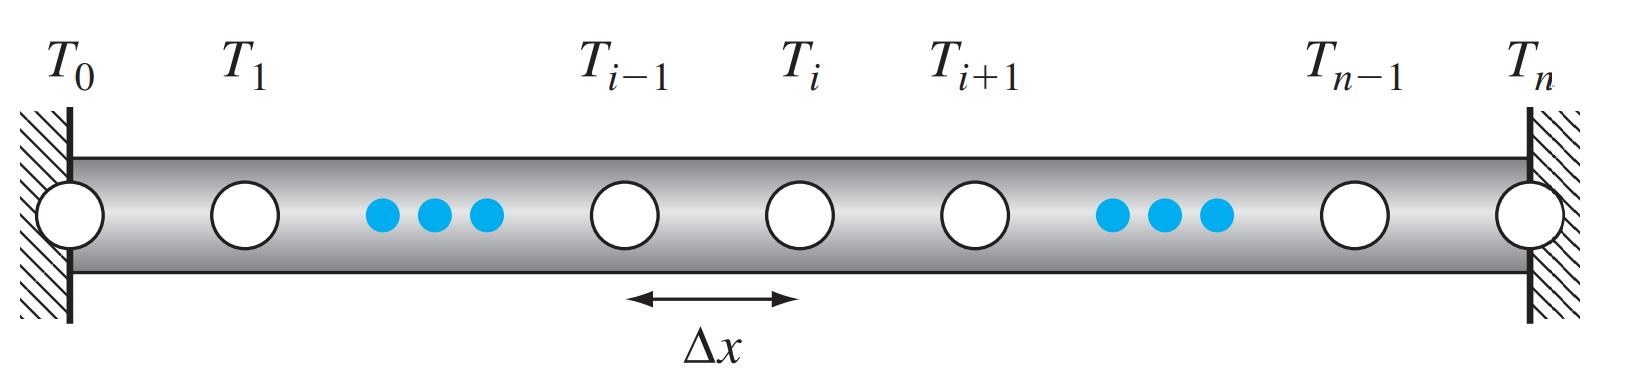
\includegraphics[scale=0.3]{fig_24_8}
   \caption{\textsf{In order to implement the finite-difference approach, the heated rod is divided into a series of
   nodes.}}\label{fig:fig_24_8}
\end{figure}

\noindent The solution domain is first divided into a series of nodes (Fig. 24.8). At each node, finite-difference approximations can be written for the derivatives in the equation. For example, at node $i$, the second derivative can be represented by (Fig. 21.5):

\begin{equation}
    \tag{24.15}
    \frac{d^{2} T}{d x^{2}}=\frac{T_{i-1}-2 T_{i}+T_{i+1}}{\Delta x^{2}}
\end{equation}

\noindent This approximation can be substituted into Eq. (24.14) to give
$$
\frac{T_{i-1}-2 T_{i}+T_{i+1}}{\Delta x^{2}}+h^{\prime}\left(T_{\infty}-T_{i}\right)=0
$$
Thus, the differential equation has been converted into an algebraic equation. Collecting terms gives
\begin{equation}
    \tag{24.16}
    -T_{i-1}+\left(2+h^{\prime} \Delta x^{2}\right) T_{i}-T_{i+1}=h^{\prime} \Delta x^{2} T_{\infty}
\end{equation}

\noindent This equation can be written for each of the $n-1$ interior nodes of the rod. The first and last nodes $T_{0}$ and $T_{n}$, respectively, are specified by the boundary conditions. Therefore, the problem reduces to solving $n-1$ simultaneous linear algebraic equations for the $n-1$ unknowns.

Before providing an example, we should mention two nice features of Eq. (24.16). First, observe that since the nodes are numbered consecutively, and since each equation consists of a node $(i)$ and its adjoining neighbors $(i-1$ and $i+1)$, the resulting set of linear algebraic equations will be tridiagonal. As such, they can be solved with the efficient algorithms that are available for such systems (recall Sec. 9.4).

Further, inspection of the coefficients on the left-hand side of Eq. (24.16) indicates that the system of linear equations will also be diagonally dominant. Hence, convergent solutions can also be generated with iterative techniques like the Gauss-Seidel method (Sec. 12.1).

\begin{exmp}
    \textbf{Finite-Difference Approximation of Boundary-Value Problems}

    \noindent\textit{Problem statement.} Use the finite-difference approach to solve the same problem as in
    Examples 24.1 and 24.2. Use four interior nodes with a segment length of $\Delta x$ = 2 m.\vspace{\medskipamount}

    \noindent\textbf{Solution.} Employing the parameters in Example 24.1 and $\Delta x$ = 2 m, we can write 
    Eq. (24.16) for each of the rod's interior nodes. For example, for node 1:
    $$
    -T_0+2.2T_1-T_2=40
    $$
    Substituting the boundary condition $T_0$ = 300 gives
    $$
    2.2T_1-T_2=340
    $$
    After writing Eq. (24.16) for the other interior nodes, the equations can be assembled in
    matrix form as 
    \begin{equation} \nonumber
        \left[\begin{array}{cccc}
        2.2 & -1 & 0 & 0 \\
        -1 & 2.2 & -1 & 0 \\
        0 & -1 & 2.2 & -1 \\
        0 & 0 & -1 & 2.2
        \end{array}\right]\left\{\begin{array}{l}
        T_{1} \\
        T_{2} \\
        T_{3} \\
        T_{4}
        \end{array}\right\}=\left\{\begin{array}{c}
        340 \\
        40 \\
        40 \\
        440
        \end{array}\right\}
    \end{equation}

    Notice that the matrix is both tridiagonal and diagonally dominant.

    MATLAB can be used to generate the solution:\vspace*{\smallskipamount}

    \noindent\texttt{>> A=[2.2 -1 0 0;\\
    -1 2.2 -1 0;\\
    0 -1 2.2 -1;\\
    0 0 -1 2.2];\\
    >> b=[340 40 40 440]';\\
    >> T=A\b}\vspace*{\smallskipamount}

    \noindent\texttt{T =\\
    \hspace*{\smallskipamount} 283.2660\\
    \hspace*{\smallskipamount} 283.1853\\
    \hspace*{\smallskipamount} 299.7416\\
    \hspace*{\smallskipamount} 336.2462}
\end{exmp}

Table 24.1 provides a comparison between the analytical solution (Eq. 24.7) and the 
numerical solutions obtained with the shooting method (Example 24.2) and the finite-difference method (Example 24.5). Note that although there are some discrepancies, the
numerical approaches agree reasonably well with the analytical solution. Further, the biggest
discrepancy occurs for the finite-difference method due to the coarse node spacing we used
in Example 24.5. Better agreement would occur if a finer nodal spacing had been used.

\begin{figure}[H]
    \centering
    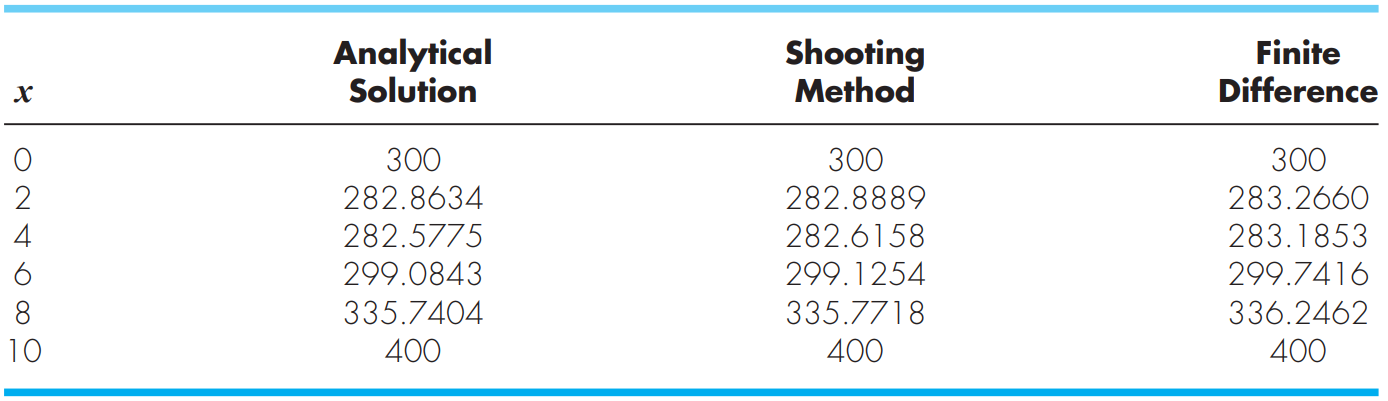
\includegraphics[scale=0.4]{table_24_1}
   \caption{\textsf{In order to implement the finite-difference approach, the heated rod is divided into a series of
   nodes.}}\label{tab:table_24_1} %TODO numerowanie obrazków "Table"
\end{figure}

\subsection{Derivative Boundary Conditions}

\noindent As mentioned in our discussion of the shooting method, the fixed or \textit{Dirichlet boundary condition} is but one of several types that are used in engineering and science. A common alternative, called the \textit{Neumann boundary condition}, is the case where the derivative is given.

\begin{figure}[H]
    \centering
    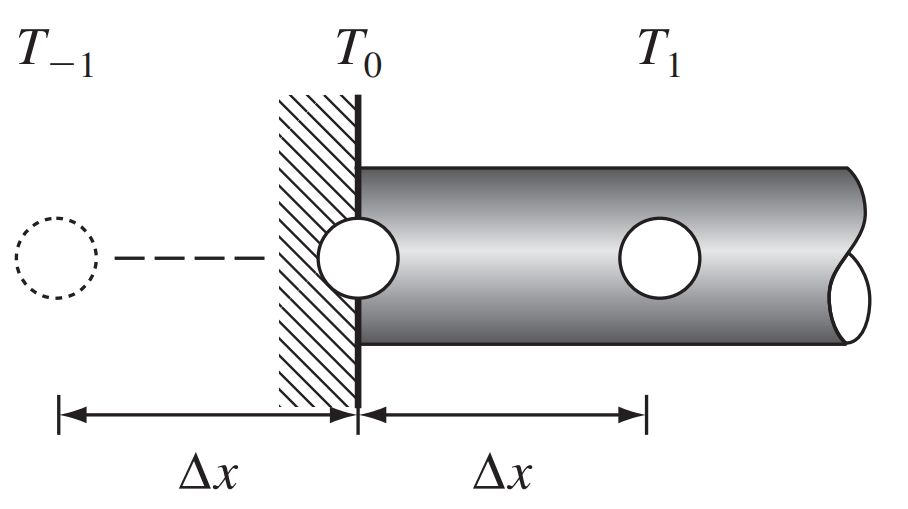
\includegraphics[scale=0.3]{fig_24_9}
   \caption{\textsf{A boundary node at the left end of a heated rod. To approximate the derivative at the boundary,
   an imaginary node is located a distance $\Delta x$ to the left of the rod's end.}}\label{fig:fig_24_9}
\end{figure}

We can use the heated rod introduced earlier in this chapter to demonstrate how a derivative boundary condition can be incorporated into the finite-difference approach:
$$
0=\frac{d^{2} T}{d x^{2}}+h^{\prime}\left(T_{\infty}-T\right)
$$
However, in contrast to our previous discussions, we will prescribe a derivative boundary condition at one end of the rod:
$$
\begin{aligned}
&\frac{d T}{d x}(0)=T_{a}^{\prime} \\
&T(L)=T_{b}
\end{aligned}
$$
Thus, we have a derivative boundary condition at one end of the solution domain and a fixed boundary condition at the other.

Just as in the previous section, the rod is divided into a series of nodes and a finitedifference version of the differential equation (Eq. 24.16) is applied to each interior node. However, because its temperature is not specified, the node at the left end must also be included. Fig. $24.9$ depicts the node (0) at the left edge of a heated plate for which the derivative boundary condition applies. Writing Eq. (24.16) for this node gives
\begin{equation}
    \tag{24.17}
    -T_{-1}+\left(2+h^{\prime} \Delta x^{2}\right) T_{0}-T_{1}=h^{\prime} \Delta x^{2} T_{\infty}
\end{equation}

Notice that an imaginary node (-1) lying to the left of the rod's end is required for this equation. Although this exterior point might seem to represent a difficulty, it actually serves as the vehicle for incorporating the derivative boundary condition into the problem. This is done by representing the first derivative in the $x$ dimension at $(0)$ by the centered difference (Eq. 4.25):
$$
\frac{d T}{d x}=\frac{T_{1}-T_{-1}}{2 \Delta x}
$$
which can be solved for
$$
T_{-1}=T_{1}-2 \Delta x \frac{d T}{d x}
$$

Now we have a formula for $T_{-1}$ that actually reflects the impact of the derivative. It can be substituted into Eq. (24.17) to give
\begin{equation}
    \tag{24.18}
    \left(2+h^{\prime} \Delta x^{2}\right) T_{0}-2 T_{1}=h^{\prime} \Delta x^{2} T_{\infty}-2 \Delta x \frac{d T}{d x}
\end{equation}

\noindent Consequently, we have incorporated the derivative into the balance.

A common example of a derivative boundary condition is the situation where the end of the rod is insulated. In this case, the derivative is set to zero. This conclusion follows directly from Fourier's law (Eq. 24.5), because insulating a boundary means that the heat flux (and consequently the gradient) must be zero. The following example illustrates how the solution is affected by such boundary conditions.

\begin{exmp}
    \textbf{Incorporating Derivative Boundary Conditions}

    \noindent\textit{Problem Statement.} Generate the finite-difference solution for a $10-\mathrm{m}$ rod with $\Delta x=2 \mathrm{~m}, h^{\prime}=0.05 \mathrm{~m}^{-2}, T_{\infty}=200 \mathrm{~K}$, and the boundary conditions: $T_{a}^{\prime}=0$ and $T_{b}=400 \mathrm{~K}$. Note that the first condition means that the slope of the solution should approach zero at the rod's left end. Aside from this case, also generate the solution for $d T / d x=-20$ at $x=0$.

    \noindent\textbf{Solution.} Equation (24.18) can be used to represent node 0 as
    $$
    2.2 T_{0}-2 T_{1}=40
    $$
    We can write Eq. (24.16) for the interior nodes. For example, for node 1 ,
    $$
    -T_{0}+2.2 T_{1}-T_{2}=40
    $$
    A similar approach can be used for the remaining interior nodes. The final system of equations can be assembled in matrix form as
    $$
    \left[\begin{array}{ccccc}
    2.2 & -2 & & & \\
    -1 & 2.2 & -1 & & \\
    & -1 & 2.2 & -1 & \\
    & & -1 & 2.2 & -1 \\
    & & & -1 & 2.2
    \end{array}\right]\left\{\begin{array}{l}
    T_{0} \\
    T_{1} \\
    T_{2} \\
    T_{3} \\
    T_{4}
    \end{array}\right\}=\left\{\begin{array}{c}
    40 \\
    40 \\
    40 \\
    40 \\
    440
    \end{array}\right\}
    $$
    These equations can be solved for
    $$
    \begin{aligned}
    &T_{0}=243.0278 \\
    &T_{1}=247.3306 \\
    &T_{2}=261.0994 \\
    &T_{3}=287.0882 \\
    &T_{4}=330.4946
    \end{aligned}
    $$
    As displayed in Fig. 24.10, the solution is flat at $x=0$ due to the zero derivative condition and then curves upward to the fixed condition of $T=400$ at $x=10$.

    \begin{figure}[H]
        \centering
        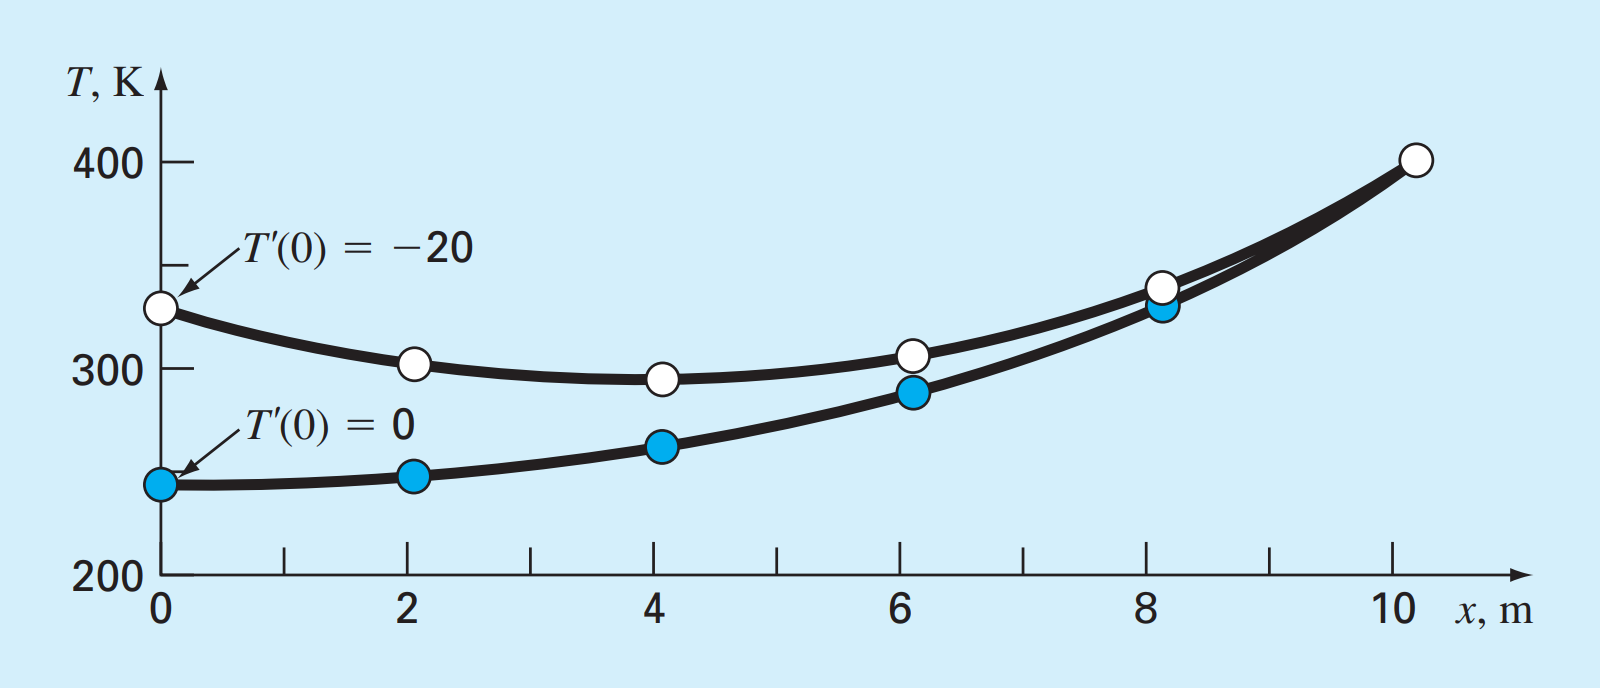
\includegraphics[scale=0.3]{fig_24_10}
       \caption{\textsf{The solution of a second-order ODE with a derivative boundary condition at one end and a fixed boundary condition at the other. Two cases are shown reflecting different derivative values at x = 0.}}\label{fig:fig_24_10}
    \end{figure}

    For the case where the derivative at $x=0$ is set to $-20$, the simultaneous equations are
    $$
    \left[\begin{array}{ccccc}
    2.2 & -2 & & & \\
    -1 & 2.2 & -1 & & \\
    & -1 & 2.2 & -1 & \\
    & & -1 & 2.2 & -1 \\
    & & & -1 & 2.2
    \end{array}\right]\left\{\begin{array}{l}
    T_{0} \\
    T_{1} \\
    T_{2} \\
    T_{3} \\
    T_{4}
    \end{array}\right\}=\left\{\begin{array}{c}
    120 \\
    40 \\
    40 \\
    40 \\
    440
    \end{array}\right\}
    $$
    which can be solved for
    $$
    \begin{aligned}
    &T_{0}=328.2710 \\
    &T_{1}=301.0981 \\
    &T_{2}=294.1448 \\
    &T_{3}=306.0204 \\
    &T_{4}=339.1002
    \end{aligned}
    $$
    As in Fig. 24.10, the solution at $x=0$ now curves downward due to the negative derivative we imposed at the boundary.
\end{exmp}\vspace*{\medskipamount}

\subsection{Finite-Difference Approaches for Nonlinear ODEs}

\noindent For nonlinear ODEs, the substitution of finite differences yields a system of nonlinear simultaneous equations. Thus, the most general approach to solving such problems is to use
root-location methods for systems of equations such as the Newton-Raphson method described in Section 12.2.2. Although this approach is certainly feasible, an adaptation of
successive substitution can sometimes provide a simpler alternative.

The heated rod with convection and radiation introduced in Example 24.4 provides a
nice vehicle for demonstrating this approach,

\begin{equation} \nonumber
    0=\frac{d^{2} T}{d x^{2}}+h^{\prime}\left(T_{\infty}-T\right)+\sigma^{\prime^{\prime}}\left(T_{\infty}^{4}-T^{4}\right)
\end{equation}

\noindent We can convert this differential equation into algebraic form by writing it for a node $i$ and substituting Eq. (24.15) for the second derivative:
$$
0=\frac{T_{i-1}-2 T_{i}+T_{i+1}}{\Delta x^{2}}+h^{\prime}\left(T_{\infty}-T_{i}\right)+\sigma^{\prime^{\prime}}\left(T_{\infty}^{4}-T_{i}^{4}\right)
$$
Collecting terms gives
$$
-T_{i-1}+\left(2+h^{\prime} \Delta x^{2}\right) T_{i}-T_{i+1}=h^{\prime} \Delta x^{2} T_{\infty}+\sigma^{\prime \prime} \Delta x^{2}\left(T_{\infty}^{4}-T_{i}^{4}\right)
$$

Notice that although there is a nonlinear term on the right-hand side, the left-hand side is expressed in the form of a linear algebraic system that is diagonally dominant. If we assume that the unknown nonlinear term on the right is equal to its value from the previous iteration, the equation can be solved for
\begin{equation}
    \tag{24.19}
    T_{i}=\frac{h^{\prime} \Delta x^{2} T_{\infty}+\sigma^{\prime^{\prime}} \Delta x^{2}\left(T_{\infty}^{4}-T_{i}^{4}\right)+T_{i-1}+T_{i+1}}{2+h^{\prime} \Delta x^{2}}
\end{equation}

\noindent As in the Gauss-Seidel method, we can use Eq. (24.19) to successively calculate the temperature of each node and iterate until the process converges to an acceptable tolerance. Although this approach will not work for all cases, it converges for many ODEs derived from physically based systems. Hence, it can sometimes prove useful for solving problems routinely encountered in engineering and science.\vspace*{\smallskipamount}

\begin{exmp}
    \textbf{The Finite-Difference Method for Nonlinear ODEs}
    \noindent\textit{Problem Statement.} Use the finite-difference approach to simulate the temperature of a heated rod subject to both convection and radiation:
    $$
    0=\frac{d^{2} T}{d x^{2}}+h^{\prime}\left(T_{\infty}-T\right)+\sigma^{\prime^{\prime}}\left(T_{\infty}^{4}-T^{4}\right)
    $$
    where $\sigma^{\prime}=2.7 \times 10^{-9} \mathrm{~K}^{-3} \mathrm{~m}^{-2}, L=10 \mathrm{~m}, h^{\prime}=0.05 \mathrm{~m}^{-2}, T_{\infty}=200 \mathrm{~K}, T(0)=300 \mathrm{~K}$, and $T(10)=400 \mathrm{~K}$. Use four interior nodes with a segment length of $\Delta x=2 \mathrm{~m}$. Recall that we solved the same problem with the shooting method in Example 24.4.
    
    \noindent\textbf{Solution.} Using Eq. (24.19) we can successively solve for the temperatures of the rod's interior nodes. As with the standard Gauss-Seidel technique, the initial values of the interior nodes are zero with the boundary nodes set at the fixed conditions of $T_{0}=300$ and $T_{5}=400$. The results for the first iteration are
    $$
    \begin{aligned}
    &T_{1}=\frac{0.05(2)^{2} 200+2.7 \times 10^{-9^{\prime}}(2)^{2}\left(200^{4}-0^{4}\right)+300+0}{2+0.05(2)^{2}}=159.2432 \\
    &T_{2}=\frac{0.05(2)^{2} 200+2.7 \times 10^{-9^{\prime}}(2)^{2}\left(200^{4}-0^{4}\right)+159.2432+0}{2+0.05(2)^{2}}=97.9674
    \end{aligned}
    $$

    \begin{figure}[H]
        \centering
        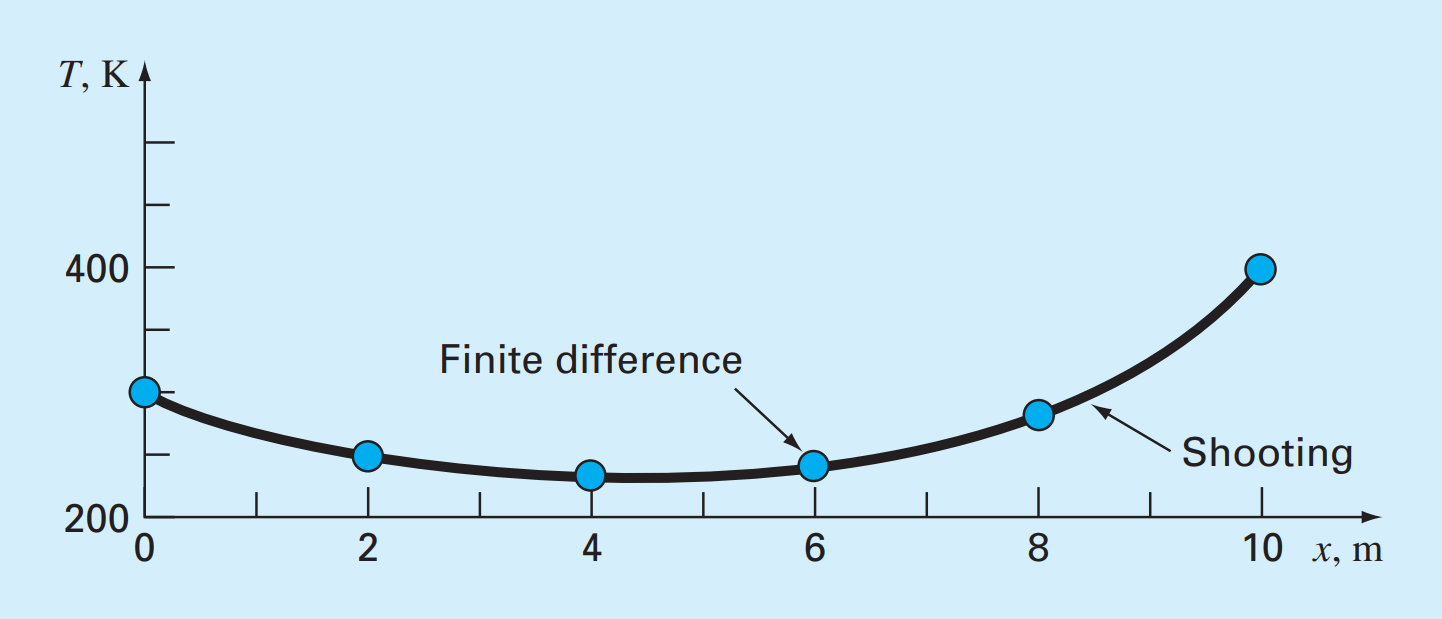
\includegraphics[scale=0.4]{fig_24_11}
       \caption{\textsf{The filled circles are the result of using the finite-difference method to solve a nonlinear problem. The line generated with the shooting method in Example 24.4 is shown for comparison.}}\label{fig:fig_24_11}
    \end{figure}

    $$
    \begin{aligned}
    T_{3} &=\frac{0.05(2)^{2} 200+2.7 \times 10^{-9^{\prime}}(2)^{2}\left(200^{4}-0^{4}\right)+97.9674+0}{2+0.05(2)^{2}}=70.4461 \\
    T_{4} &=\frac{0.05(2)^{2} 200+2.7 \times 10^{-9^{\prime}}(2)^{2}\left(200^{4}-0^{4}\right)+70.4461+400}{2+0.05(2)^{2}}=226.8704
    \end{aligned}
    $$
    The process can be continued until we converge on the final result:
    $$
    \begin{aligned}
    &T_{0}=300 \\
    &T_{1}=250.4827 \\
    &T_{2}=236.2962 \\
    &T_{3}=245.7596 \\
    &T_{4}=286.4921 \\
    &T_{5}=400
    \end{aligned}
    $$
    These results are displayed in Fig. $24.11$ along with the result generated in Example $24.4$ with the shooting method.
\end{exmp}\vspace*{2cm}

\section{Problems}
\begin{multicols}{2}
    \noindent\textbf{24.1} A steady-state heat balance for a rod can be represented as
    $$\frac{d^2}{dx^2}-0.15T=0$$
    Obtain a solution for a 10-m rod with T (0) = 240 and T(10) = 150 \textbf{(a)} analytically, \textbf{(b)} with the shooting method, and \textbf{(c)} using the finite-difference approach with $\Delta x$ = 1.\vspace{2mm}

    \noindent\textbf{24.2} Repeat Prob. 24.1 but with the right end insulated and
    the left end temperature fixed at 240.\vspace{2mm}

    \noindent\textbf{24.3} Use the shooting method to solve
    $$7 \frac{d^{2} y}{d x^{2}}-2 \frac{d y}{d x}-y+x=0$$
    with the boundary conditions y(0) = 5 and y(20) = 8.\vspace{2mm}

    \noindent\textbf{24.4} Solve Prob. 24.3 with the finite-difference approach
    using $\Delta x$ = 2.\vspace{2mm}

    \noindent\textbf{24.5} The following nonlinear differential equation was
    solved in Examples 24.4 and 24.7.\vspace{2mm}
    \begin{equation}
        \tag{P24.5}
        0=\frac{d^{2} T}{d x^{2}}+h^{\prime}\left(T_{\infty}-T\right)+\sigma^{\prime^{\prime}}\left(T_{\infty}^{4}-T^{4}\right)
    \end{equation}
    Such equations are sometimes linearized to obtain an approximate solution. This is done by employing a first-order
    Taylor series expansion to linearize the quartic term in the
    equation as
    $$\sigma^{\prime} T^{4}=\sigma^{\prime} \bar{T}^{4}+4 \sigma^{\prime} \bar{T}^{3}(T-\bar{T})$$
    where $\overline{T}$ is a base temperature about which the term is linearized. Substitute this relationship into Eq. (P24.5), and then solve the resulting linear equation with the finitedifference approach. Employ $\overline{T}=300, \Delta x=1 \mathrm{~m}$, and the parameters from Example $24.4$ to obtain your solution. Plot your results along with those obtained for the nonlinear versions in Examples $24.4$ and 24.7.\vspace{2mm}

    \noindent\textbf{24.6} Develop an M-file to implement the shooting method
    for a linear second-order ODE. Test the program by duplicating Example 24.2.\vspace{2mm}

    \noindent\textbf{24.7} Develop an M-file to implement the finite-difference
    approach for solving a linear second-order ODE with Dirichlet boundary conditions. Test it by duplicating Example 24.5.\vspace{2mm}

    \noindent\textbf{24.8} An insulated heated rod with a uniform heat source can be modeled with the \textit{Poisson equation:}
    $$\frac{d^2T}{dx^2}=-f(x)$$
    Given a heat source $f(x)=25^{\circ} \mathrm{C} / \mathrm{m}^{2}$ and the boundary conditions $T(x=0)=40^{\circ} \mathrm{C}$ and $T(x=10)=200^{\circ} \mathrm{C}$, solve for the temperature distribution with \textbf{(a)} the shooting method and \textbf{(b)} the finite-difference method ($\Delta x=2)$.\vspace{2mm}
    
    \noindent\textbf{24.9} Repeat Prob. $24.8$, but for the following spatially varying heat source: $f(x)=0.12 x^{3}-2.4 x^{2}+12 x$.\vspace{2mm}

    \noindent\textbf{24.10} The temperature distribution in a tapered conical cooling fin (Fig. P24.10) is described by the following differential equation, which has been nondimensionalized:
    $$
    \frac{d^{2} u}{d x^{2}}+\left(\frac{2}{x}\right)\left(\frac{d u}{d x}-p u\right)=0
    $$
    where $u=$ temperature $(0 \leq u \leq 1), x=$ axial distance $(0 \leq x \leq 1)$, and $p$ is a nondimensional parameter that describes the heat transfer and geometry:
    $$
    p=\frac{h L}{k} \sqrt{1+\frac{4}{2 m^{2}}}
    $$
    where $h=$ a heat transfer coefficient, $k=$ thermal conductivity, $L=$ the length or height of the cone, and $m=$ the slope of the cone wall. The equation has the boundary conditions:
    $$
    u(x=0)=0 \quad u(x=1)=1
    $$
    Solve this equation for the temperature distribution using finite-difference methods. Use second-order accurate finitedifference formulas for the derivatives. Write a computer program to obtain the solution and plot temperature versus axial distance for various values of $p=10,20,50$, and 100.
    \begin{figure}[H]
        \centering
        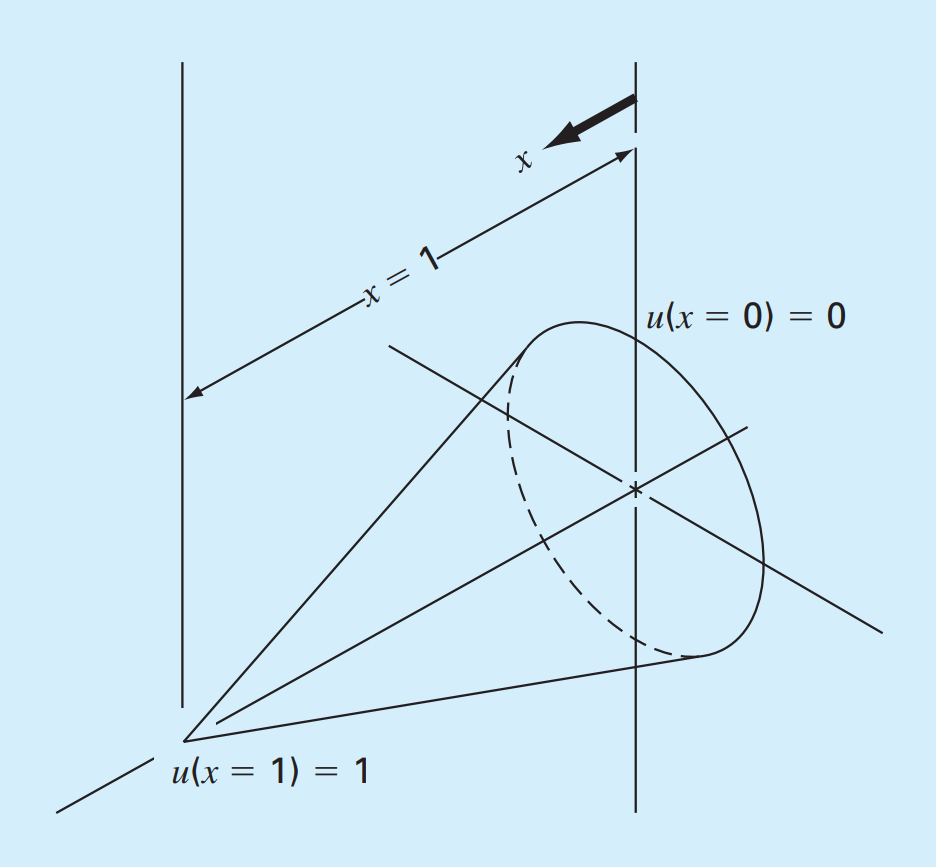
\includegraphics[scale=0.35]{fig_P_24_10}
        \caption{}
       \label{fig:fig_P_24_10} %TODO wyświetlanie odpowiedniego(!) podpisu obrazka
    \end{figure}\vspace{2mm}

    \noindent\textbf{24.11} 24.11 Compound $A$ diffuses through a 4-cm-long tube and reacts as it diffuses. The equation governing diffusion with reaction is
    $$
    D \frac{d^{2} A}{d x^{2}}-k A=0
    $$
    At one end of the tube $(x=0)$, there is a large source of $A$ that results in a fixed concentration of $0.1 \mathrm{M}$. At the other end of the tube there is a material that quickly absorbs any $A$, making the concentration $0 \mathrm{M}$. If $D=1.5 \times 10^{-6} \mathrm{~cm}^{2} / \mathrm{s}$ and $k=5 \times 10^{-6} \mathrm{~s}^{-1}$, what is the concentration of $A$ as a function of distance in the tube?\vspace{2mm}

    \noindent\textbf{24.12} The following differential equation describes the steady-state concentration of a substance that reacts with first-order kinetics in an axially dispersed plug-flow reactor (Fig. P24.12):
    $$
    D \frac{d^{2} c}{d x^{2}}-U \frac{d c}{d x}-k c=0
    $$
    where $D=$ the dispersion coefficient $\left(\mathrm{m}^{2} / \mathrm{hr}\right), c=$ concentration (mol/L), $x=$ distance $(\mathrm{m}), U=$ the velocity $(\mathrm{m} / \mathrm{hr})$, and $k=$ the reaction rate (/hr). The boundary conditions can be formulated as
    $$
    \begin{aligned}
    &U c_{\text {in }}=U c(x=0)-D \frac{d c}{d x}(x=0) \\
    &\frac{d c}{d x}(x=L)=0
    \end{aligned}
    $$
    where $c_{\text {in }}=$ the concentration in the inflow $(\mathrm{mol} / \mathrm{L}), L=$ the length of the reactor (m). These are called Danckwerts boundary conditions.
    
    Use the finite-difference approach to solve for concentration as a function of distance given the following parameters: $D=5000 \mathrm{~m}^{2} / \mathrm{hr}, U=100 \mathrm{~m} / \mathrm{hr}, k=2 / \mathrm{hr}, L=100 \mathrm{~m}$, and $c_{\mathrm{in}}=100 \mathrm{~mol} / \mathrm{L}$. Employ centered finite-difference approximations with $\Delta x=10 \mathrm{~m}$ to obtain your solutions. Compare your numerical results with the analytical solution:
    $c=\frac{U c_{\text {in }}}{\left(U-D \lambda_{1}\right) \lambda_{2} e^{\lambda_{2} L}-\left(U-D \lambda_{2}\right) \lambda_{1} e^{\lambda_{1} L}}$
    $\times\left(\lambda_{2} e^{\lambda_{2} L} e^{\lambda_{1} x}-\lambda_{1} e^{\lambda_{1} L} e^{\lambda_{2} x}\right)$
    where
    $$
    \frac{\lambda_{1}}{\lambda_{2}}=\frac{U}{2 D}\left(1 \pm \sqrt{1+\frac{4 k D}{U^{2}}}\right)
    $$

    \begin{figure}[H]
        \centering
        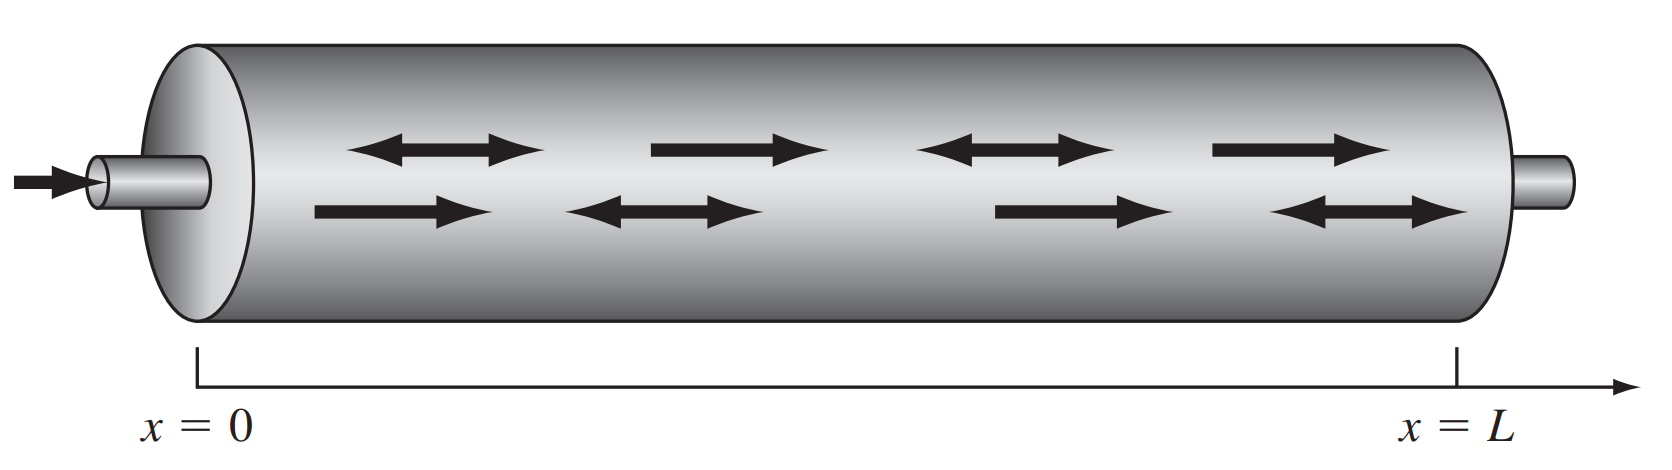
\includegraphics[scale=0.18]{fig_P_24_12}
        \caption{}
       \label{fig:fig_P_24_12} %TODO wyświetlanie odpowiedniego(!) podpisu obrazka
    \end{figure}\vspace{2mm}

    \noindent\textbf{24.13} A series of first-order, liquid-phase reactions create a desirable product (B) and an undesirable byproduct (C):
    $$
    \mathrm{A} \stackrel{k_{1}}{\rightarrow} \mathrm{B} \stackrel{k_{2}}{\rightarrow} \mathrm{C}
    $$
    If the reactions take place in an axially dispersed plug-flow reactor (Fig. P24.12), steady-state mass balances can be used to develop the following second-order ODEs:
    $$
    \begin{aligned}
    &D \frac{d^{2} c_{a}}{d x^{2}}-U \frac{d c_{a}}{d x}-k_{1} c_{a}=0 \\
    &D \frac{d^{2} c_{b}}{d x^{2}}-U \frac{d c_{b}}{d x}+k_{1} c_{a}-k_{2} c_{b}=0 \\
    &D \frac{d^{2} c_{c}}{d x^{2}}-U \frac{d c_{c}}{d x}+k_{2} c_{b}=0
    \end{aligned}
    $$
    Use the finite-difference approach to solve for the concentration of each reactant as a function of distance given: $D=$ $0.1 \mathrm{~m}^{2} / \mathrm{min},\ U=1 \mathrm{~m} / \mathrm{min},\ k_{1}=3 / \mathrm{min},\ k_{2}=1 / \mathrm{min},\ L=$ $0.5 \mathrm{~m},\ c_{a \text {,in }}=10 \mathrm{~mol} / \mathrm{L}$.
    Employ centered finite-difference approximations with $\Delta x=0.05 \mathrm{~m}$ to obtain your solutions and assume Danckwerts boundary conditions as described in Prob. 24.12. Also, compute the sum of the reactants as a function of distance. Do your results make sense?\vspace{2mm}

    \noindent\textbf{24.14} A biofilm with a thickness $L_{f}(\mathrm{~cm})$, grows on the surface of a solid (Fig. P24.14). After traversing a diffusion layer of thickness $L(\mathrm{~cm})$, a chemical compound $A$ diffuses into the biofilm where it is subject to an irreversible firstorder reaction that converts it to a product $B$.

    Steady-state mass balances can be used to derive the following ordinary differential equations for compound $A$ :
    \begin{equation} \nonumber
        D \frac{d^{2} c_{a}}{d x^{2}}=0 \quad 0 \leq x<L
    \end{equation}\vspace*{\smallskipamount} 
    \begin{equation}\nonumber
        D_{f} \frac{d^{2} c_{a}}{d x^{2}}-k c_{a}=0 \quad L \leq x<L+L_{f}
    \end{equation}

    \noindent where $D=$ the diffusion coefficient in the diffusion layer $=$ $0.8 \mathrm{~cm}^{2} / \mathrm{d}, D_{f}=$ the diffusion coefficient in the biofilm $=$ $0.64 \mathrm{~cm}^{2} / \mathrm{d}$, and $k=$ the first-order rate for the conversion of $A$ to $B=0.1 / \mathrm{d}$. The following boundary conditions hold: $c_{a}=c_{a 0} \quad$ at $x=0$ $\frac{d c_{a}}{d x}=0 \quad$ at $x=L+L_{f}$
    where $c_{a 0}=$ the concentration of $\mathrm{A}$ in the bulk liquid $=$ $100 \mathrm{~mol} / \mathrm{L}$. Use the finite-difference method to compute the steady-state distribution of A from $x=0$ to $L+L_{f}$, where $L=0.008 \mathrm{~cm}$ and $L_{f}=0.004 \mathrm{~cm}$. Employ centered finite differences with $\Delta x=0.001 \mathrm{~cm}$.

    \begin{figure}[H]
        \centering
        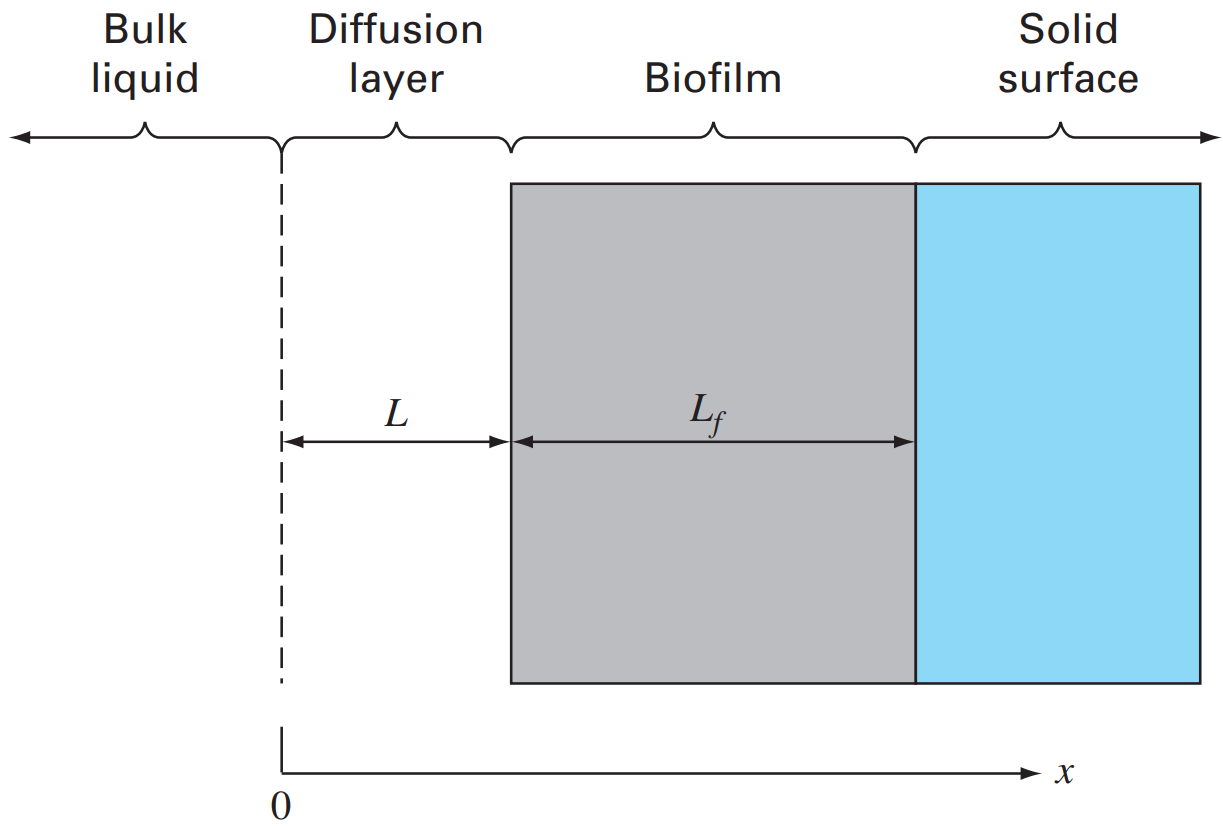
\includegraphics[scale=0.2]{fig_P_24_14}
        \caption{\textsf{A biofilm growing on a solid surface.}}
       \label{fig:fig_P_24_14} %TODO wyświetlanie odpowiedniego(!) podpisu obrazka
    \end{figure}\vspace{2mm}

    \noindent\textbf{24.15} A cable is hanging from two supports at $A$ and $B$ (Fig. P24.15). The cable is loaded with a distributed load whose magnitude varies with $x$ as
    $$
    w=w_{o}\left[1+\sin \left(\frac{\pi x}{2 l_{A}}\right)\right]
    $$
    where $w_{o}=450 \mathrm{~N} / \mathrm{m}$. The slope of the cable $(d y / d x)=0$ at $x=0$, which is the lowest point for the cable. It is also the point where the tension in the cable is a minimum of $T_{o}$. The differential equation which governs the cable is
    $$
    \frac{d^{2} y}{d x^{2}}=\frac{w_{o}}{T_{o}}\left[1+\sin \left(\frac{\pi x}{2 l_{A}}\right)\right]
    $$
    Solve this equation using a numerical method and plot the shape of the cable ( $y$ versus $x$ ). For the numerical solution, the value of $T_{o}$ is unknown, so the solution must use an iterative technique, similar to the shooting method, to converge on a correct value of $h_{A}$ for various values of $T_{\sigma}$.

    \begin{figure}[H]
        \centering
        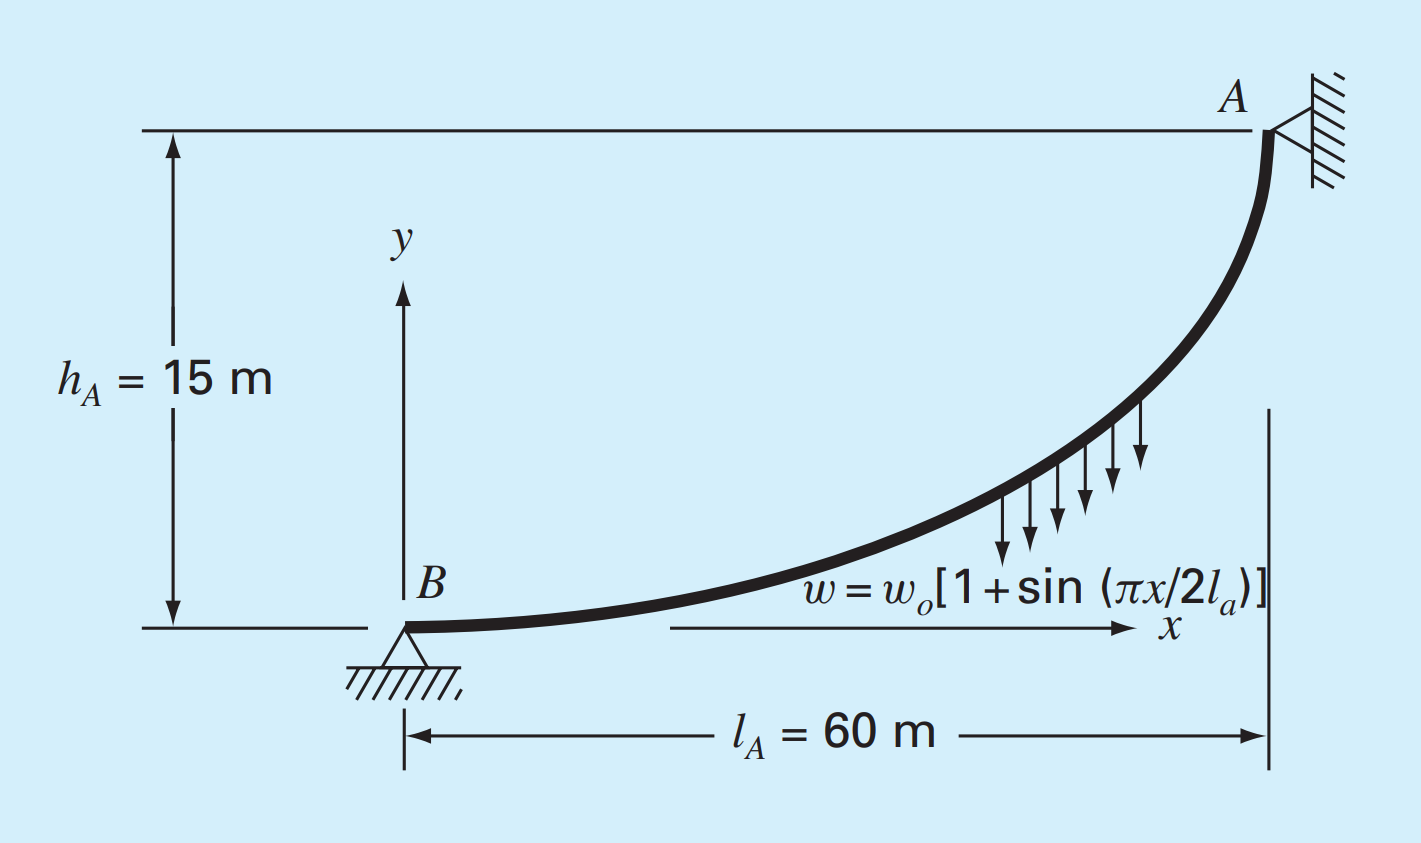
\includegraphics[scale=0.22]{fig_P_24_15}
        \caption{}
       \label{fig:fig_P_24_15} %TODO wyświetlanie odpowiedniego(!) podpisu obrazka
    \end{figure}\vspace{2mm}

    \noindent\textbf{24.16} The basic differential equation of the elastic curve for a simply supported, uniformly loaded beam (Fig. P24.16) is given as
    $$
    E I \frac{d^{2} y}{d x^{2}}=\frac{w L x}{2}-\frac{w x^{2}}{2}
    $$
    where $E=$ the modulus of elasticity, and $I=$ the moment of inertia. The boundary conditions are $y(0)=y(L)=0$. Solve for the deflection of the beam using (a) the finite-difference approach $(\Delta x=0.6 \mathrm{~m})$ and (b) the shooting method. The following parameter values apply: $E=200 \mathrm{GPa}, I=$ $30,000 \mathrm{~cm}^{4}, w=15 \mathrm{kN} / \mathrm{m}$, and $L=3 \mathrm{~m}$. Compare your numerical results to the analytical solution:
    $$
    y=\frac{w L x^{3}}{12 E I}-\frac{w x^{4}}{24 E I}-\frac{w L^{3} x}{24 E I}
    $$
    \begin{figure}[H]
        \centering
        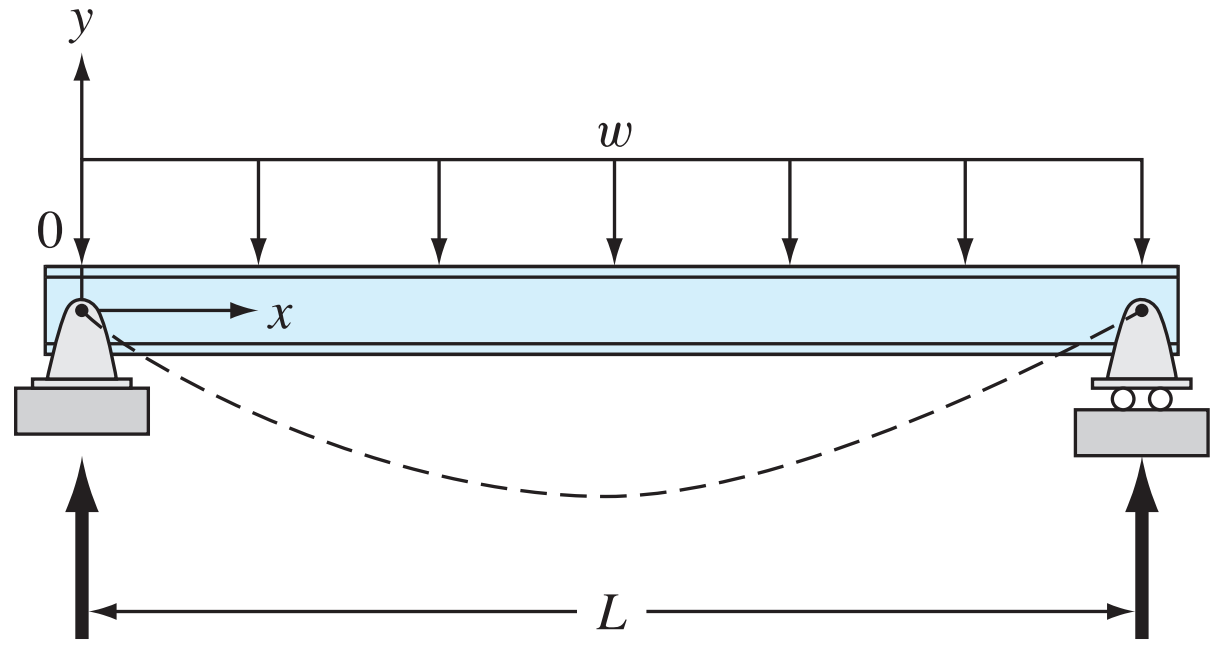
\includegraphics[scale=0.25]{fig_P_24_16}
        \caption{}
       \label{fig:fig_P_24_16} %TODO wyświetlanie odpowiedniego(!) podpisu obrazka
    \end{figure}\vspace{2mm}

    \noindent\textbf{24.17} In Prob. 24.16, the basic differential equation of the elastic curve for a uniformly loaded beam was formulated as
    $$
    E I \frac{d^{2} y}{d x^{2}}=\frac{w L x}{2}-\frac{w x^{2}}{2}
    $$
    Note that the right-hand side represents the moment as a function of $x$. An equivalent approach can be formulated in terms of the fourth derivative of deflection as
    $$
    E I \frac{d^{4} y}{d x^{4}}=-w
    $$
    For this formulation, four boundary conditions are required. For the supports shown in Fig. P24.16, the conditions are that the end displacements are zero, $y(0)=y(L)=0$, and that the end moments are zero, $y^{\prime \prime}(0)=y^{\prime \prime}(L)=0$.
    Solve for the deflection of the beam using the finite-difference approach $(\Delta x=0.6 \mathrm{~m})$. The following parameter values apply: $E=$ $200 \mathrm{GPa}, I=30,000 \mathrm{~cm}^{4}, w=15 \mathrm{kN} / \mathrm{m}$, and $L=3 \mathrm{~m}$. Compare your numerical results with the analytical solution given in Prob. 24.16.\vspace{2mm}

    \noindent\textbf{24.18} Under a number of simplifying assumptions, the steady-state height of the water table in a one-dimensional, unconfined groundwater aquifer (Fig. P24.18) can be modeled with the following second-order ODE:
    $$
    K \bar{h} \frac{d^{2} h}{d x^{2}}+N=0
    $$
    where $x=$ distance $(\mathrm{m}), K=$ hydraulic conductivity $(\mathrm{m} / \mathrm{d})$, $h=$ height of the water table $(\mathrm{m}), \bar{h}=$ the average height of the water table $(\mathrm{m})$, and $N=$ infiltration rate $(\mathrm{m} / \mathrm{d})$.
    
    Solve for the height of the water table for $x=0$ to $1000 \mathrm{~m}$ where $h(0)=10 \mathrm{~m}$ and $h(1000)=5 \mathrm{~m}$. Use the following parameters for the calculation: $K=1 \mathrm{~m} / \mathrm{d}$ and $N=0.0001 \mathrm{~m} / \mathrm{d}$. Set the average height of the water table as the average of the boundary conditions. Obtain your solution with \textbf{(a)} the shooting method and \textbf{(b)} the finite-difference method $(\Delta x=100 \mathrm{~m})$.

    \begin{figure}[H]
        \centering
        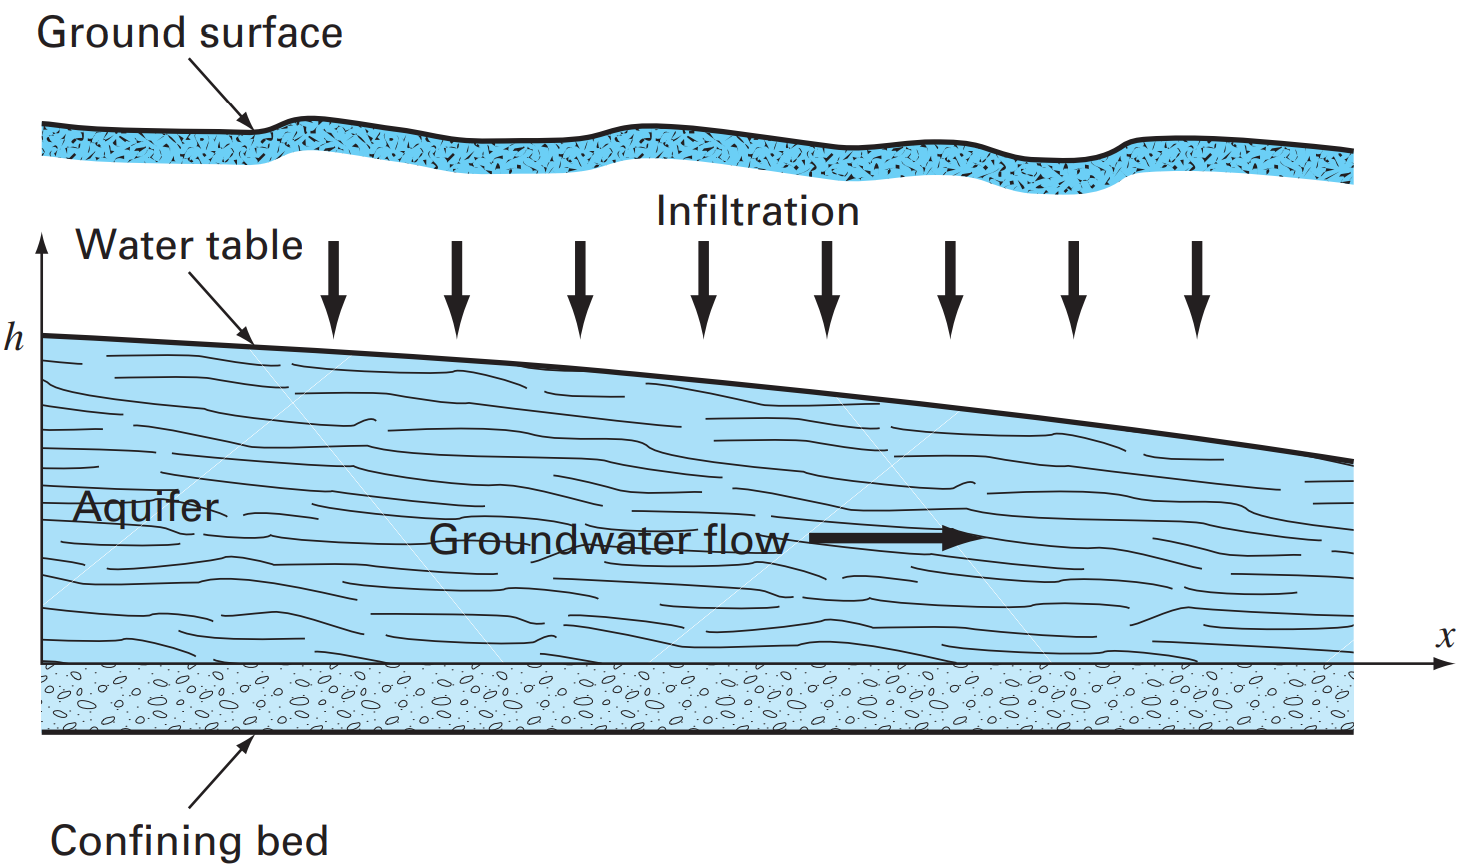
\includegraphics[scale=0.22]{fig_P_24_18}
       \caption{\textsf{An unconfined or "phreatic" aquifer.}}\label{fig:fig_P_24_18}
    \end{figure}\vspace{2mm}

    \noindent\textbf{24.19} 24.19 In Prob. 24.18, a linearized groundwater model was used to simulate the height of the water table for an unconfined aquifer. A more realistic result can be obtained by using the following nonlinear ODE:
    $$
    \frac{d}{d x}\left(K h \frac{d h}{d x}\right)+N=0
    $$
    where $x=$ distance $(\mathrm{m}), K=$ hydraulic conductivity $(\mathrm{m} / \mathrm{d})$, $h=$ height of the water table $(\mathrm{m})$, and $N=$ infiltration rate $(\mathrm{m} / \mathrm{d})$. Solve for the height of the water table for the same case as in Prob. 24.18.
    That is, solve from $x=0$ to $1000 \mathrm{~m}$ with $h(0)=10 \mathrm{~m},\ h(1000)=5 \mathrm{~m},\ K=1 \mathrm{~m} / \mathrm{d}$, and $N=0.0001 \mathrm{~m} / \mathrm{d}$. Obtain your solution with \textbf{(a)} the shooting method and \textbf{(b)} the finite-difference method $(\Delta x=100 \mathrm{~m})$.\vspace{2mm}

    \noindent\textbf{24.20} Just as Fourier's law and the heat balance can be employed to characterize temperature distribution, analogous relationships are available to model field problems in other areas of engineering. For example, electrical engineers use a similar approach when modeling electrostatic fields. Under a number of simplifying assumptions, an analog of Fourier's law can be represented in one-dimensional form as
    $$
    D=-\varepsilon \frac{d V}{d x}
    $$
    where $D$ is called the electric flux density vector, $\varepsilon=$ permittivity of the material, and $V=$ electrostatic potential. Similarly, a Poisson equation (see Prob. 24.8) for electrostatic fields can be represented in one dimension as
    $$
    \frac{d^{2} V}{d x^{2}}=-\frac{\rho_{v}}{\varepsilon}
    $$
    where $\rho_{v}=$ charge density. Use the finite-difference technique with $\Delta x=2$ to determine $V$ for a wire where $V(0)=$ $1000,\ V(20)=0,\ \varepsilon=2,\ L=20$, and $\rho_{v}=30$.\vspace{2mm}

    \noindent\textbf{24.21} $24.21$ Suppose that the position of a falling object is governed by the following differential equation:
    $$
    \frac{d^{2} x}{d t^{2}}+\frac{c}{m} \frac{d x}{d t}-g=0
    $$
    where $c=$ a first-order drag coefficient $=12.5 \mathrm{~kg} / \mathrm{s},\ m=$ mass $=70 \mathrm{~kg}$, and $g=$ gravitational acceleration $=9.81 \mathrm{~m} / \mathrm{s}^{2}$. Use the shooting method to solve this equation for the boundary conditions:
    $$
    \begin{aligned}
    &x(0)=0 \\
    &x(12)=500
    \end{aligned}
    $$\vspace{2mm}

    \noindent\textbf{24.22} As in Fig. P24.22, an insulated metal rod has a fixed temperature $\left(T_{0}\right)$ boundary condition at its left end. On it right end, it is joined to a thin-walled tube filled with water through which heat is conducted. The tube is insulated at its right end and convects heat with the surrounding fixedtemperature air $\left(T_{\infty}\right)$. The convective heat flux at a location $x$ along the tube $\left(\mathrm{W} / \mathrm{m}^{2}\right)$ is represented by
    $$
    J_{\text {conv }}=h\left(T_{\infty}-T_{2}(x)\right)
    $$
    where $h=$ the convection heat transfer coefficient $\left[\mathrm{W} /\left(\mathrm{m}^{2} \cdot \mathrm{K}\right)\right]$. Employ the finite-difference method with $\Delta x=0.1 \mathrm{~m}$ to compute the temperature distribution for the case where both the rod and tube are cylindrical with the same radius $r(\mathrm{~m})$. Use the following parameters for your analysis:
    $L_{\text {rod }}=0.6 \mathrm{~m},\ L_{\text {tube }}=0.8 \mathrm{~m},\ T_{0}=400 \mathrm{~K},\ T_{\infty}=300 \mathrm{~K}$, $r=3 \mathrm{~cm},\ \rho_{1}=7870 \mathrm{~kg} / \mathrm{m}^{3},\ C_{p 1}=447 \mathrm{~J} /(\mathrm{kg} \cdot \mathrm{K}),\ k_{1}=80.2$ $\mathrm{W} /(\mathrm{m} \cdot \mathrm{K})$,
    $\rho_{2}=1000 \mathrm{~kg} / \mathrm{m}^{3},\ C_{p 2}=4.18 \mathrm{~kJ} /(\mathrm{kg} \cdot \mathrm{K}),\ k_{2}=$ $0.615 \mathrm{~W} /(\mathrm{m} \cdot \mathrm{K})$, and $h=3000 \mathrm{~W} /\left(\mathrm{m}^{2} \cdot \mathrm{K}\right)$. The subscripts designate the rod (1) and the tube (2).

    \begin{figure}[H]
        \centering
        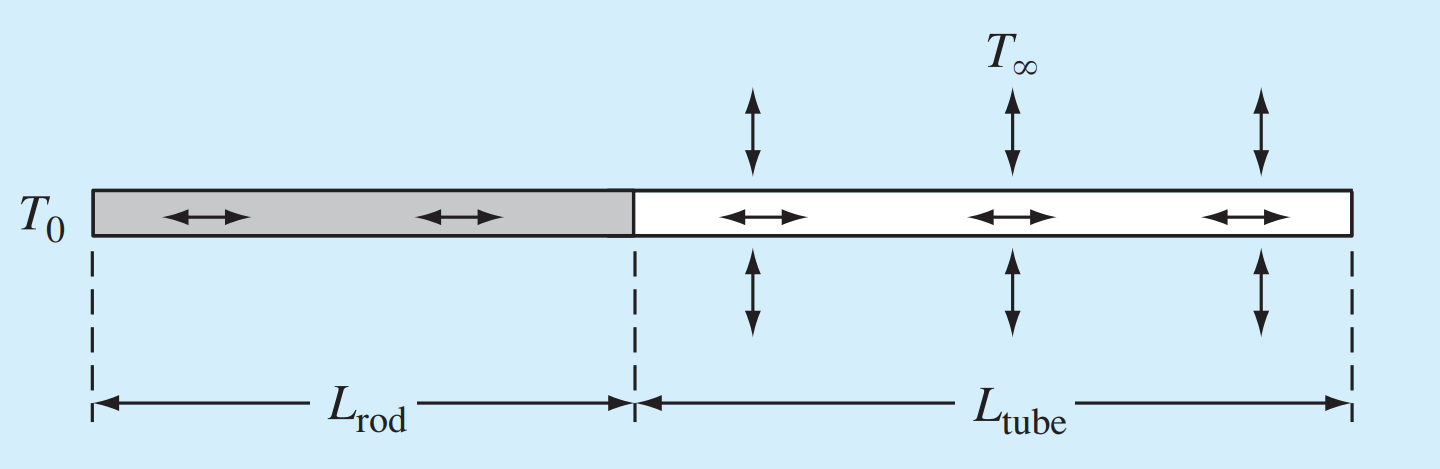
\includegraphics[scale=0.21]{fig_P_24_22}
       \caption{}\label{fig:fig_P_24_22}
    \end{figure}\vspace{2mm}

    \noindent\textbf{24.23} Perform the same calculation as in Prob. 24.22, butfor the case where the tube is also insulated (i.e., no convection) and the right-hand wall is held at a fixed boundary temperature of 200 K. 

    
\end{multicols}

\end{document}